\documentclass[12pt,a4paper]{report}
\usepackage[utf8]{inputenc}
\usepackage[T1]{fontenc}
\usepackage{lmodern}
\usepackage[brazil]{babel}
\usepackage[a4paper,margin=2.5cm]{geometry}
\usepackage{graphicx}
\usepackage{booktabs}
\usepackage{amsmath}
\usepackage{float}
\usepackage{longtable}
\usepackage[round,authoryear]{natbib}
\usepackage[hidelinks]{hyperref}

\graphicspath{{../outputs/figures/}}
\setlength{\parskip}{0.45em}
\renewcommand{\arraystretch}{1.15}

\begin{document}
\hypersetup{pageanchor=false}

\begin{titlepage}
\centering
\vspace*{1cm}
{\scshape\large Fundação Getulio Vargas \\ Escola de Economia de São Paulo (EESP)\par}
\vspace{2.5cm}
{\huge\bfseries Forecasting consolidado da exposição de gestoras a ações\par}
\vspace{0.8cm}
{\Large Evidência do mercado brasileiro de fundos, 2016--2021\par}
\vspace{3cm}
{\Large João Paulo Zangrandi\par}
\vspace{0.5cm}
{\large Orientador: Prof.\ Maurício Ferraresi Junior\par}
\vfill
{\large São Paulo \\ \today\par}
\end{titlepage}

\hypersetup{pageanchor=true}
\pagenumbering{roman}

\chapter*{Resumo}
\addcontentsline{toc}{chapter}{Resumo}
Este trabalho mede e prevê a exposição consolidada das gestoras brasileiras a ações, inspirado pela literatura
de \emph{demand-based asset pricing}. A unidade empírica central é gestora $\times$ mês $\times$ ação:
para cada ação, observa-se mês a mês quais gestoras aumentaram ou reduziram exposição e testa-se se a
exposição futura pode ser prevista a partir do histórico da própria gestora e do comportamento do restante do
mercado, isto é, das demais gestoras. O núcleo empírico usa as bases CONS e SH da CVM para construir um
painel consolidado de exposição em R\$ e US\$, por gestora e por ação, com validação inicial em ITUB4 e
extensão para todos os tickers identificáveis.

O resultado central de dados é que a exposição institucional é concentrada em \emph{blue chips}, exatamente
os ativos em que a literatura de demanda e propriedade comum sugere maior relevância para preços e risco. No
forecasting, a variação mensal é difícil de prever; o nível da exposição em valor mostra reversão à média em
ITUB4 e em algumas ações muito líquidas, mas uma especificação consolidada com todas as ações elegíveis,
restante do mercado ($n-1$), fator comum e validação fora da amostra não supera o \emph{random walk}. A
quantidade estimada de ITUB4, construída com preço B3/COTAHIST, entra como robustez para separar preço de
quantidade. A CDA Bloco~2 não substitui esse núcleo consolidado: ela é tratada em apêndice técnico, com
detalhe, para reconstruir a rede fundo$\to$fundo apagada pela CONS, avaliar aninhamento, testar
circularidade e fundamentar extensões futuras com modelos de grafo.

\noindent\textbf{Palavras-chave:} demand-based asset pricing; fundos de investimento; exposição em ações;
forecasting; redes; CVM.

\tableofcontents

\clearpage
\pagenumbering{arabic}

\chapter{Introdução}

O objetivo deste trabalho é medir e prever a exposição consolidada das gestoras brasileiras a ações. A
pergunta empírica nasce de uma ideia simples: se investidores institucionais têm demandas persistentes por
ativos, então carteiras observadas podem conter informação sobre comportamento futuro. A literatura de
\emph{demand-based asset pricing} fornece a motivação: preços não são determinados apenas por fundamentos
agregados, mas também pela demanda de investidores com restrições, preferências e mandatos específicos
\citep{koijenyogo2019,gabaixkoijen2021}.

O caso brasileiro é adequado para esse exercício porque a CVM disponibiliza bases públicas de fundos. A CONS
permite observar a composição consolidada das carteiras e a SH permite associar cada fundo à sua gestora e
ao seu patrimônio líquido. Essas bases permitem medir exposição em valor, em R\$ e US\$, que é a medida mais
direta de escala econômica e risco patrimonial. A previsão é feita de forma consolidada por gestora: para
cada ação e mês, mede-se quem aumentou ou reduziu exposição; para cada gestora, usa-se seu próprio histórico
e o comportamento das demais gestoras, o ``restante do mercado'' ou $n-1$, para prever exposição futura.

A quantidade estimada de ações é construída para ITUB4 com o fechamento oficial mensal da B3
\citep{b3_cotahist}. Ela é mantida como robustez conceitual, pois ajuda a separar efeito de preço de mudança
aproximada de quantidade,
mas a medida principal de exposição do trabalho permanece em valor. A CDA Bloco~2, por sua vez, entra como
apêndice técnico: a CONS é consolidada e apaga o caminho de fundos investindo em fundos; a CDA recupera esse
caminho e permite visualizar a rede fundo$\to$fundo. No desenho atual, não se prevê o grafo em si. O alvo da
previsão é a exposição consolidada. A rede é uma forma de representar interconexões e uma possível camada
futura de features ou modelos de grafo.

O trabalho responde a cinco perguntas:
\begin{enumerate}
\item Como medir a exposição das gestoras a ações em R\$ e US\$, com tratamento consistente de empréstimos de
ações e grupos econômicos?
\item A exposição futura de uma gestora pode ser prevista a partir do próprio histórico e do restante do
mercado?
\item A diferença entre exposição em valor e quantidade estimada muda a interpretação de demanda?
\item A evidência inicial de ITUB4 se generaliza para outras ações?
\item Como a rede fundo$\to$fundo, reconstruída pela CDA em apêndice, qualifica a interpretação de risco e
prepara uma extensão com modelos de grafo?
\end{enumerate}

\begin{figure}[H]\centering
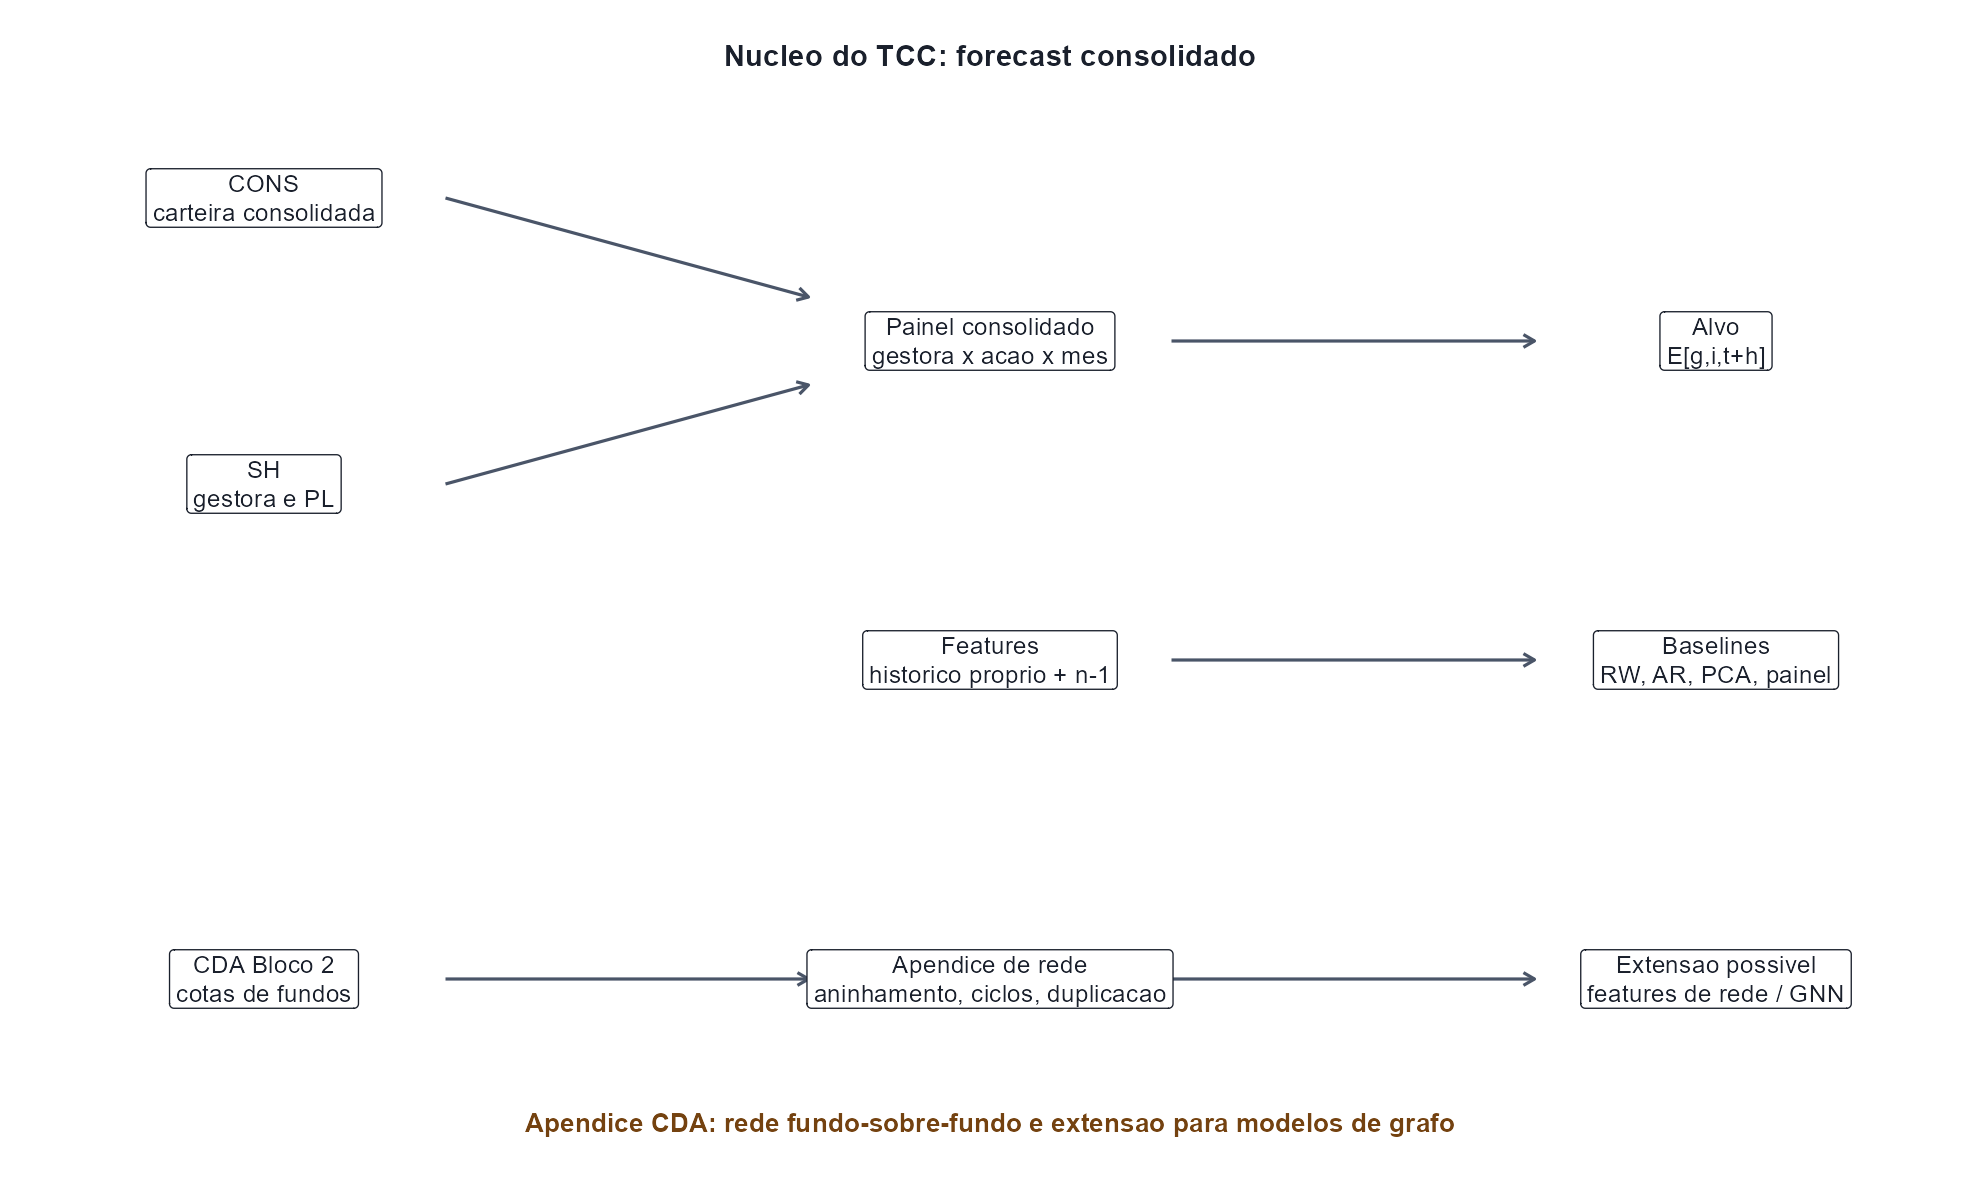
\includegraphics[width=0.92\textwidth]{research_design_graph.png}
\caption{Desenho empírico: núcleo consolidado e apêndice de rede.}
\label{fig:design}
\end{figure}

Assim, a CDA não entra como base alternativa à CONS. As duas têm funções diferentes. A CONS mede a exposição
final em ações e sustenta o forecasting consolidado; a CDA recupera o caminho de fundos sobre fundos e
documenta uma camada de rede que pode ser usada para risco, de-duplicação e extensões de graph learning. Os
detalhes de tratamento da CDA ficam no Apêndice~\ref{ap:cda}.

\chapter{Revisão Bibliográfica}

\section{Demand-based asset pricing}

\citet{koijenyogo2019} propõem um sistema de demanda por ativos no qual investidores institucionais
escolhem carteiras em função de características dos ativos, preços e restrições próprias. A contribuição
central para este TCC é tratar carteiras observadas como revelação de demanda. Em vez de olhar apenas para
retornos ou fundamentos agregados, o pesquisador usa a composição das carteiras para inferir como diferentes
investidores demandam ativos.

\citet{gabaixkoijen2021} desenvolvem a hipótese de mercados inelásticos: fluxos podem ter impacto
desproporcional sobre preços quando a demanda agregada por ações não é altamente elástica. Para este
trabalho, a implicação é direta: se gestoras concentram demanda nas mesmas ações e ajustam posições de forma
correlacionada, variações de exposição podem ser relevantes para preços e risco.

\section{Fragilidade por propriedade comum}

\citet{greenwoodthesmar2011} mostram que a estrutura de propriedade pode gerar fragilidade de preços.
Ativos detidos por investidores sujeitos a choques semelhantes tendem a ficar mais vulneráveis, pois vendas
ou compras correlacionadas podem amplificar movimentos. No nosso contexto, as ações \emph{crowded}, detidas
por muitas gestoras, são candidatas naturais a esse tipo de fragilidade.

\section{Métodos de previsão e fatores}

O uso de PCA e análise fatorial segue a lógica de que a demanda institucional pode ter fatores comuns. A
referência metodológica usada no projeto é \citet{artesbarroso2023}. Empiricamente, o PCA é estimado apenas
na janela de treino para evitar vazamento de informação.

Redes neurais em grafo são mencionadas como possibilidade metodológica, com referência introdutória em
\citet{sanchezlengeling2021}. A motivação é direta: se fundos estão conectados por relações de cotas, então
essa estrutura pode ser transformada em uma matriz de adjacência e usada como informação para prever
exposição. Ainda assim, o alvo deste TCC não é prever a topologia da rede. O alvo é a exposição consolidada
por gestora e ação. A rede CDA é documentada como apêndice e como extensão metodológica possível.

\section{Plataformas de investimento}

O working paper \emph{Replicant Investment Platforms}, do Prof.\ Maurício Ferraresi Junior
\citep{ferraresi_replicant}, é mantido como referência provisória a confirmar. Ele é relevante para a
interpretação de plataformas e vasos de investimento entre fundos, exatamente o tipo de estrutura que a CDA
permite observar empiricamente. Como a citação exata ainda precisa ser confirmada, este eixo fica tratado com
cautela.

\chapter{Metodologia e Dados}

\section{Bases do núcleo empírico consolidado}

O núcleo do trabalho usa duas bases públicas da CVM e uma base auxiliar de preços da B3:

\paragraph{CONS.} A composição consolidada de carteiras tem granularidade fundo $\times$ mês $\times$ ativo.
No período 2016--2021, a amostra tratada contém aproximadamente 21,1 milhões de linhas. A base é 100\%
classificada como ``Ações'', porque a consolidação da CVM dissolve cotas de fundos em ativos finais. Os
valores de \texttt{Valor\_Ativo\_mil} estão em formato americano, com ponto decimal e eventual notação
científica.

\paragraph{SH.} A série histórica dos fundos tem granularidade fundo $\times$ dia e traz informações de
gestora, classificação, nome do fundo e patrimônio líquido. O PL vem em formato brasileiro e é convertido
para número com parser específico.

\paragraph{B3/COTAHIST.} A CONS não informa quantidade de ações. Para converter a posição em ITUB4 de valor
para quantidade estimada, usa-se o fechamento diário oficial da B3/COTAHIST, mercado à vista
(\texttt{TPMERC=010}), selecionando o último pregão de cada mês. A amostra de preços cobre os 72 meses entre
janeiro de 2016 e dezembro de 2021, sem lacunas mensais.

A ligação entre CONS e SH é feita por \texttt{Código} (CONS) igual a \texttt{COD\_FUNDO} (SH), mantendo o
mesmo CNPJ e a mesma data de competência mensal. A revisão de qualidade encontrou apenas 2 fundos-mês da
CONS sem correspondência no SH.

\section{Tratamentos de dados}

Os principais tratamentos são:
\begin{itemize}
\item normalização de CNPJ para dígitos;
\item parser separado para números em formato americano (CONS) e dinheiro em formato brasileiro (SH);
\item remoção de linhas exatamente duplicadas na CONS, definidas por mesmo CNPJ, código, data, ativo e valor;
\item extração de ticker terminal a partir do nome do ativo;
\item classificação das variantes de exposição em direta, cedida e obrigação;
\item consolidação de gestoras por grupo econômico via regras de texto;
\item conversão de R\$ para US\$ com PTAX de fim de mês (BCB SGS série~1);
\item conversão auxiliar de valor de ITUB4 para quantidade estimada de ações com fechamento mensal B3/COTAHIST;
\item construção de deltas mensais apenas quando os meses são consecutivos.
\end{itemize}

A duplicata exata da CONS é um ponto importante. A revisão profunda encontrou cerca de 0,2\% de linhas
exatamente repetidas, com impacto de aproximadamente 0,01\% nos totais. A correção preserva lotes legítimos
com valores diferentes e remove apenas cópias idênticas.

\begin{table}[H]\centering
\caption{Principais checagens de validação das bases.}
\label{tab:datavalidation}
\scriptsize
\begin{tabular}{p{4.2cm}p{6.2cm}p{3.4cm}}
\toprule
\textbf{Checagem} & \textbf{Evidência} & \textbf{Leitura} \\
\midrule
Tipo de ativo na CONS & 100\% das linhas tratadas aparecem como Ações &
Consistente com uso da CONS de ações \\
Join CONS--SH & Apenas 2 fundos-mês da CONS ficam sem SH em 2016--2021 &
Cobertura praticamente completa \\
SH sem CONS & 42.024 observações; 94,7\% são fundos não-ações &
Ausência esperada pelo recorte de ações \\
Duplicatas exatas na CONS & 32.970 linhas removidas de aproximadamente 21,1 milhões &
Impacto material desprezível, mas correção necessária \\
Painel ITUB4 & 72 meses, 42 grupos econômicos, 2.835 observações gestora-mês &
Cobertura suficiente para origem móvel \\
Preço B3 de ITUB4 & 72 meses sem lacuna; erro de reconstrução de valor $9{,}3\times10^{-10}$ mil R\$ &
Quantidade estimada valida aritmeticamente \\
CDA em apêndice & 835.694 arestas; 0 self-loops; 0 meses com ciclo em 72 &
Rede útil para risco e extensão, não para substituir a CONS \\
\bottomrule
\end{tabular}
\end{table}

\section{Definição de exposição}

Para ITUB4, há três definições:
\begin{itemize}
\item \textbf{direta}: apenas a linha direta do ativo;
\item \textbf{long}: direta mais ações cedidas em empréstimo;
\item \textbf{net}: long mais obrigações por ações recebidas em empréstimo, que entram negativas.
\end{itemize}

A definição principal é \emph{net}. No período, a soma das posições mensais em ITUB4 é R\$\,468 bi na
definição direta, R\$\,540 bi na definição long e R\$\,496 bi na definição net. A definição net gera 264
observações gestora-mês com posição líquida negativa, evidenciando a relevância do aluguel de ações.

\section{Problema preditivo consolidado}

O problema preditivo do corpo do trabalho é consolidado por gestora. Para cada gestora $g$, ação $i$ e mês
$t$, observa-se a exposição $E_{g,i,t}$ e sua variação $\Delta E_{g,i,t}$. O conjunto das demais gestoras,
$-g$, resume o comportamento do restante do mercado naquela ação. Em termos gerais, o sistema de previsão
procura usar:
\[
\widehat{E}_{g,i,t+1}
= f(E_{g,i,\leq t}, E_{-g,i,\leq t}),
\]
em que $E_{-g,i,\leq t}$ representa a informação agregada ou cruzada do restante do mercado. Neste estágio,
o trabalho implementa baselines transparentes: \emph{random walk}, AR, modelos de painel e PCA/fatores. A
CDA aparece no Apêndice~\ref{ap:cda} como camada adicional: ela permite escrever uma extensão
$f(E_{g,i,\leq t}, E_{-g,i,\leq t}, G_t)$, em que $G_t$ é o grafo fundo-sobre-fundo. Essa extensão usa o
grafo como informação, mas o alvo continua sendo a exposição consolidada, não a rede futura.

\section{Quantidade estimada de ações}

Para estudar demanda em sentido estrito, valor monetário não é suficiente. A posição em reais varia tanto por
compra e venda de ações quanto por variação de preço. Como a CONS não traz número de ações, a quantidade é
estimada por:
\[
q_{g,t}^{ITUB4} =
\frac{V_{g,t}^{ITUB4}\times 1000}{P_t^{ITUB4}},
\]
em que $V_{g,t}^{ITUB4}$ é a posição em \texttt{Valor\_Ativo\_mil} e $P_t^{ITUB4}$ é o fechamento de ITUB4
no último pregão do mês na B3/COTAHIST. A multiplicação por 1000 converte o valor da CONS de mil reais para
reais.

A mesma regra é aplicada às variantes direta, cedida e obrigação. Assim:
\[
q^{dir}=\frac{1000V^{dir}}{P},\quad
q^{long}=\frac{1000(V^{dir}+V^{ced})}{P},\quad
q^{net}=\frac{1000(V^{dir}+V^{ced}+V^{obrig})}{P}.
\]
Aqui, $dir$, $ced$ e $obrig$ indicam, respectivamente, posição direta, ações cedidas em empréstimo e
obrigações por ações recebidas em empréstimo.
A definição principal permanece \emph{net}. A validação numérica reconstrói o valor original por
$q_{g,t}^{ITUB4}P_t^{ITUB4}/1000$ com erro máximo de aproximadamente $9{,}3\times10^{-10}$ mil reais, isto
é, apenas erro de arredondamento de máquina.

Essa quantidade deve ser lida como robustez e não como substituta da exposição em valor. Ela é a melhor
aproximação possível com CONS+B3 para separar efeito de preço de mudança aproximada de demanda, mas eventos
societários que alterem mecanicamente o número de ações exigem cautela na interpretação temporal. A medida
principal do TCC permanece a exposição em valor, por ser mais direta para risco patrimonial e gerenciamento
de risco.

\section{Unidade de análise}

A unidade principal é a gestora consolidada por grupo econômico. Essa decisão torna a análise mais legível e
reduz ruído de variações de nomes jurídicos. O painel ITUB4 tem 2.835 observações gestora-mês, cobrindo 42
grupos econômicos e 72 meses.

\section{Avaliação preditiva}

As previsões usam origem móvel com janela expansível. Em cada origem, o modelo é estimado apenas com dados
até o mês $t$ e prevê $t+h$. A janela mínima de treino é sempre de 36 meses. Essa escolha foi fixada antes
da leitura dos resultados e não foi flexibilizada por especificação, por alvo ou por modelo. Depois do mês
36, a janela apenas se expande: o exercício não testa janelas alternativas para escolher a que melhora o
resultado.

O benchmark é o \emph{random walk}: para a variação, a previsão é $\widehat{\Delta}=0$; para o nível, a
previsão é $\widehat{y}_{t+h}=y_t$. As métricas são:
\[
RMSE_m=\sqrt{\frac{1}{N}\sum_{j=1}^N e_{m,j}^2},\qquad
MAE_m=\frac{1}{N}\sum_{j=1}^N |e_{m,j}|,
\]
em que $e_{m,j}=y_j-\widehat{y}_{m,j}$ é o erro do modelo $m$. A \emph{skill} de RMSE é:
\[
\text{Skill}_{m}=100\times\frac{RMSE_{RW}-RMSE_m}{RMSE_{RW}}.
\]
Assim, valor positivo significa que o modelo reduziu erro contra o \emph{random walk}; valor negativo
significa que piorou. O acerto de direção mede a fração de previsões em que o sinal previsto de mudança
coincide com o sinal realizado.

Para ITUB4, os testes de significância reportados nas tabelas são diagnósticos fora da amostra: um teste
$t$ pareado da diferença de perda quadrática entre o modelo e o \emph{random walk}, e um teste binomial para
o acerto de direção contra 50\%. No painel consolidado amplo, a inferência usa \emph{bootstrap} por data de
origem, preservando a dependência transversal entre gestoras e ações observadas no mesmo mês. PCA e fatores
são sempre estimados somente na janela de treino, sem usar informação futura. A análise em valor é a
especificação principal; a análise em quantidade estimada é uma robustez para ITUB4.

\begin{table}[H]\centering
\caption{Protocolo dos testes de previsão.}
\label{tab:forecastprotocol}
\scriptsize
\begin{tabular}{p{3.2cm}p{3.5cm}p{2.2cm}p{4.3cm}}
\toprule
\textbf{Exercício} & \textbf{Alvo} & \textbf{Horizonte} & \textbf{Inferência} \\
\midrule
Variação ITUB4 em valor & $\Delta$ posição em US\$ & 1 mês &
Teste $t$ pareado da perda quadrática; binomial de direção \\
Variação ITUB4 em quantidade & $\Delta$ quantidade estimada & 1 mês &
Teste $t$ pareado da perda quadrática; binomial de direção \\
Nível ITUB4 em valor & posição em US\$ & 1, 3 e 6 meses &
Teste $t$ pareado da perda quadrática \\
Nível ITUB4 em quantidade & quantidade estimada & 1, 3 e 6 meses &
Teste $t$ pareado da perda quadrática \\
Todas as ações, por ticker & posição em US\$ & 1 mês &
Distribuição da \emph{skill} por ação; tickers degenerados marcados \\
Painel consolidado final & posição em US\$ por gestora-ação & 1 mês &
\emph{Bootstrap} por data de origem \\
\bottomrule
\end{tabular}
\end{table}

A especificação consolidada final, implementada no script da rodada 23, usa a unidade gestora $\times$ ação
$\times$ mês. Uma ação entra na avaliação quando tem ao menos cinco gestoras com histórico suficiente; uma
gestora entra para uma ação quando aparece com ao menos 24 meses positivos. A
janela mínima de treino de 36 meses também é mantida aqui. Tickers com \emph{random walk} perfeito na
amostra fora da amostra, como eventos societários ou séries degeneradas, são excluídos da métrica de
\emph{skill}, pois o denominador do ganho relativo é zero. O AR individual é estimado como reversão à média
e tem coeficiente de persistência limitado a $[0,0{,}995]$, para evitar extrapolações explosivas em séries
curtas.

\chapter{Resultados}

\section{Exposição e quantidade em ITUB4}

O painel mostra que Itaú, Bradesco, BB, Kapitalo e Santander estão entre as maiores exposições médias a
ITUB4. A Figura~\ref{fig:pos} resume a exposição em valor, enquanto a Figura~\ref{fig:qtd} mostra a
quantidade estimada de ações. A diferença entre as duas figuras é substantiva: a primeira mistura preço e
quantidade; a segunda isola a aproximação de demanda.

\begin{figure}[H]\centering
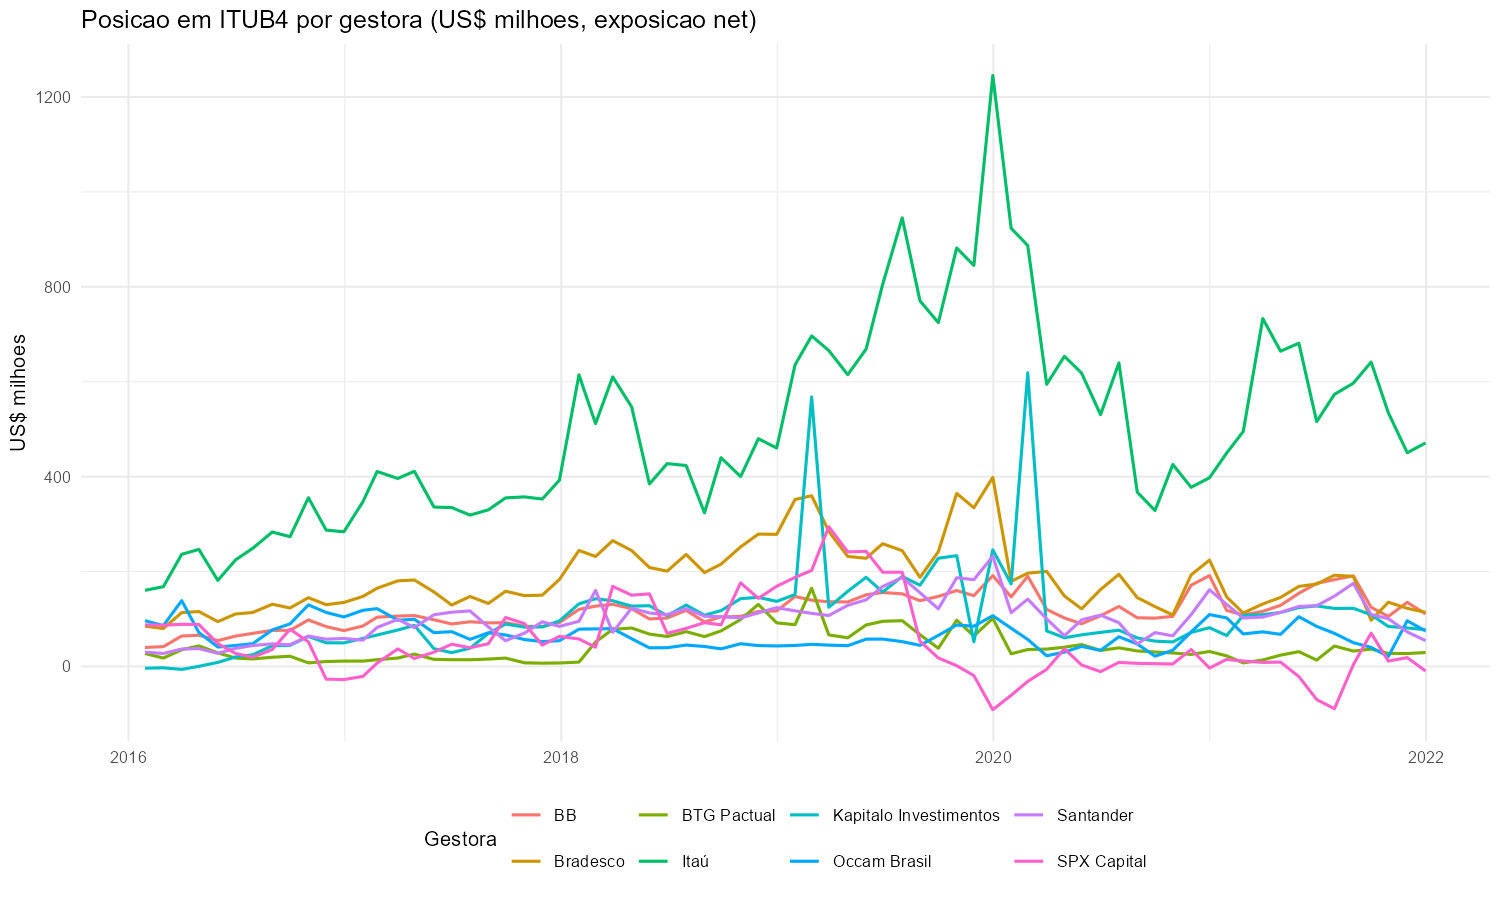
\includegraphics[width=0.88\textwidth]{pos_usd_top_gestoras.png}
\caption{Posição em ITUB4 por gestora (US\$ milhões, exposição net).}
\label{fig:pos}
\end{figure}

\begin{figure}[H]\centering
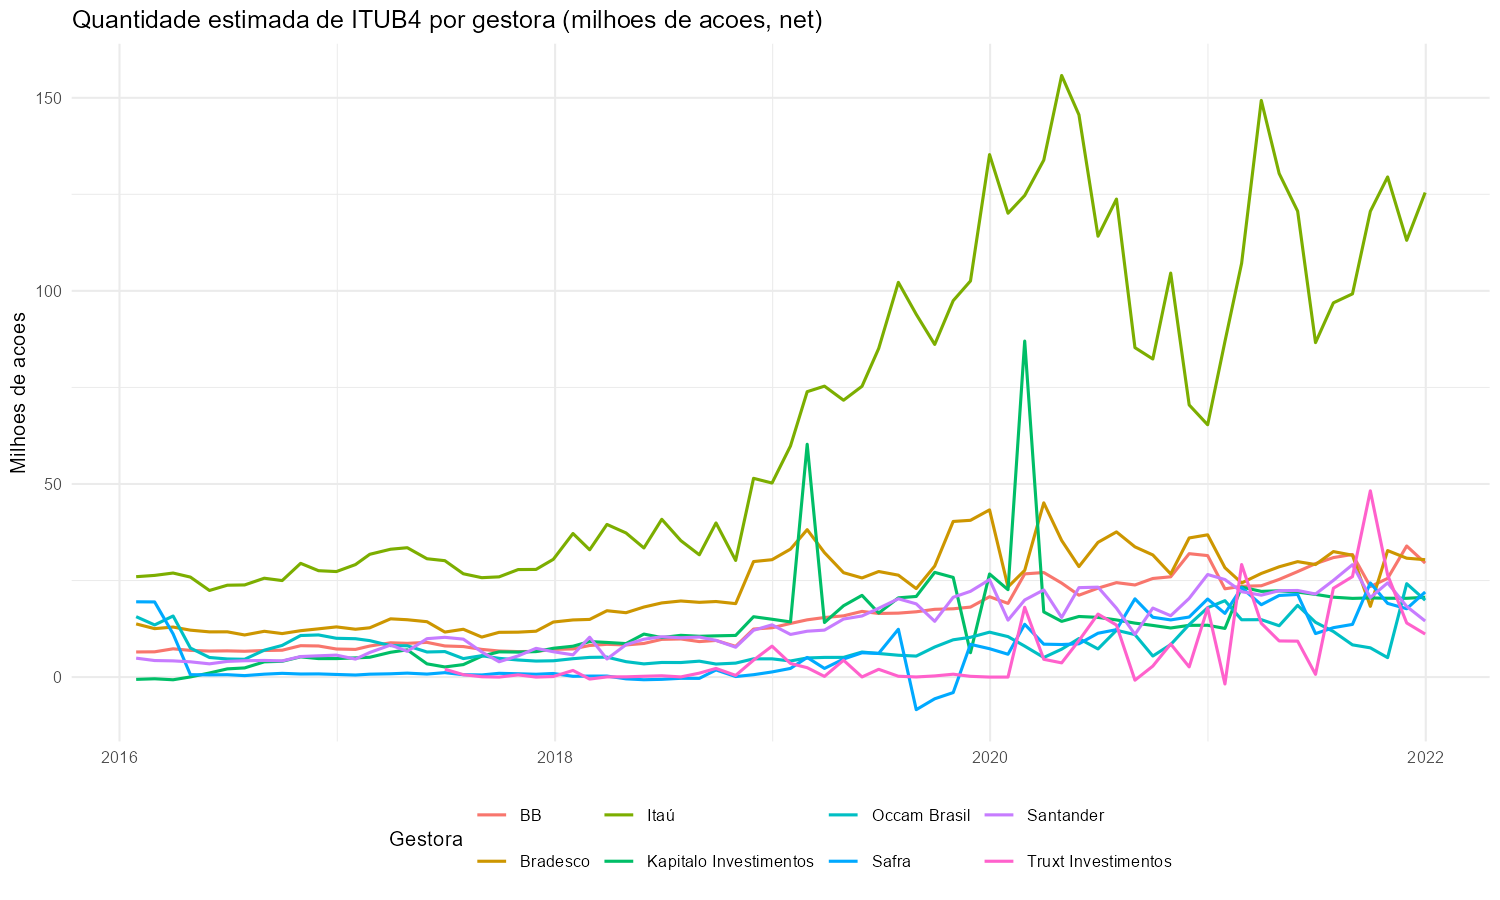
\includegraphics[width=0.88\textwidth]{qtd_itub4_top_gestoras.png}
\caption{Quantidade estimada de ITUB4 por gestora (milhões de ações, exposição net).}
\label{fig:qtd}
\end{figure}

\begin{table}[H]\centering
\caption{Definições de exposição em ITUB4: valor e quantidade estimada.}
\small
\begin{tabular}{@{}lrrrr@{}}
\toprule
\textbf{Def.} & \textbf{Valor (R\$ bi)} & \textbf{Média (US\$ mi)} &
\textbf{Qtd.\ (bi ações)} & \textbf{Qtd.\ neg.} \\
\midrule
direta & 468 & 39,0 & 14,77 & 0 \\
long   & 540 & 45,1 & 17,02 & 0 \\
net    & 496 & 41,4 & 15,71 & 264 \\
\bottomrule
\end{tabular}
\end{table}

\section{Extensão para todas as ações}

A extensão para todas as ações reconhece 836 tickers e produz um painel gestora $\times$ mês $\times$ ticker.
O resultado mais importante do núcleo CONS+SH é a concentração: as ações detidas pelo maior número de
gestoras são \emph{blue chips} como VALE3, PETR4, ITUB4, BBDC4 e EQTL3. Isso sustenta a conexão com
fragilidade por propriedade comum.

\begin{figure}[H]\centering
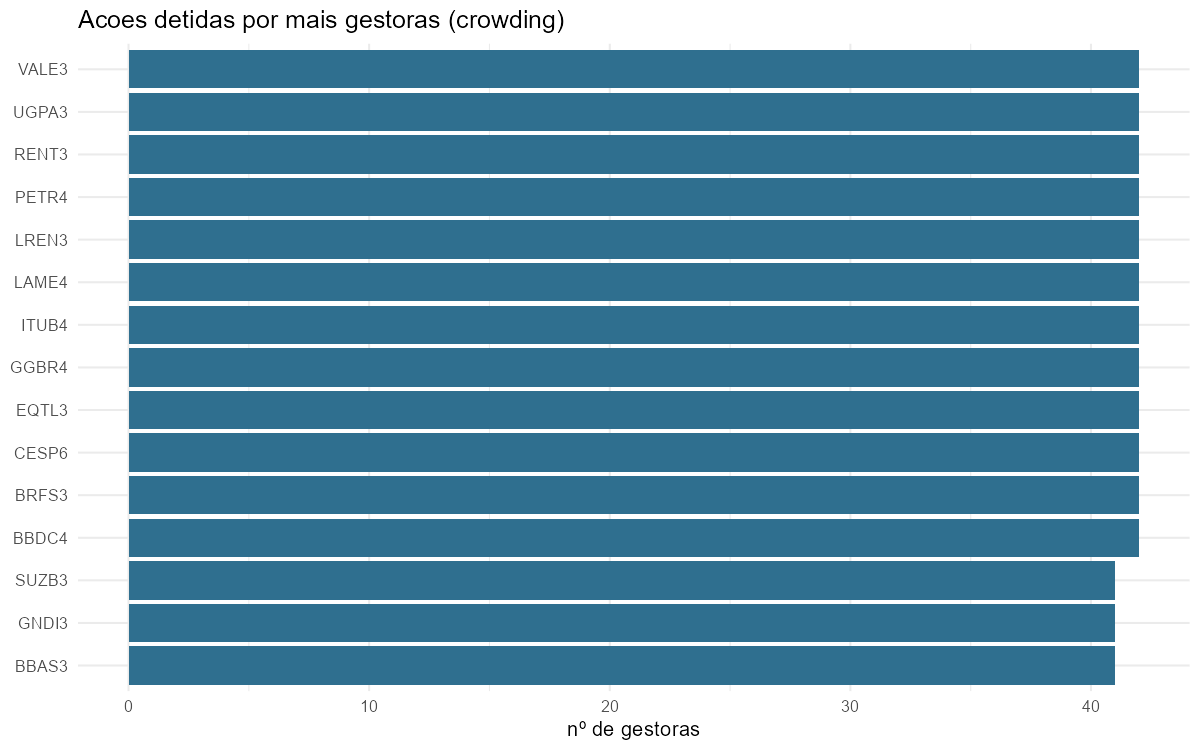
\includegraphics[width=0.82\textwidth]{stock_crowding_top15.png}
\caption{Ações detidas pelo maior número de gestoras.}
\label{fig:crowd}
\end{figure}

\section{Leitura complementar da rede}

Como a previsão do corpo do trabalho é consolidada por gestora, a rede fundo-sobre-fundo não é necessária
para construir o painel principal. Ainda assim, ela é importante para interpretar risco e para preparar uma
extensão metodológica com grafos. O Apêndice~\ref{ap:cda} documenta a CDA Bloco~2 em detalhe: leitura da
base, filtros, validações, visualizações de grafo, teste de circularidade, profundidade de aninhamento e
de-duplicação intra-gestora. A leitura correta é que a rede fundamenta uma possível camada de informação; o
alvo econométrico continua sendo a exposição consolidada por gestora e ação.

\section{Previsão da variação mensal}

Nas primeiras rodadas de forecasting, o alvo era a variação mensal da posição em US\$ para ITUB4. O
resultado é negativo e informativo. A Tabela~\ref{tab:deltausd} mostra que o AR encolhido reduz o RMSE em
0,97\%, mas o ganho não é estatisticamente robusto ($p=0{,}649$) e o MAE piora. O PCA com um fator fica
estatisticamente pior que o \emph{random walk} no teste de perda quadrática ($p=0{,}046$), e o PCA com três
fatores tem erro economicamente muito maior. A direção também não é previsível: os testes binomiais não
rejeitam 50\% de acerto.

\begin{table}[H]\centering
\caption{Variação mensal da posição de ITUB4 em US\$: testes fora da amostra.}
\label{tab:deltausd}
\scriptsize
\begin{tabular}{@{}lrrrrrr@{}}
\toprule
\textbf{Modelo} & \textbf{RMSE} & \textbf{MAE} & \textbf{Skill RMSE} &
\textbf{$p$ perda} & \textbf{Direção} & \textbf{$p$ dir.} \\
\midrule
Random walk    & 41,10 & 14,35 & 0,00\%   & --     & --     & -- \\
AR encolhido   & 40,70 & 14,61 & +0,97\%  & 0,649  & 47,8\% & 0,152 \\
AR             & 41,54 & 15,26 & -1,05\%  & 0,801  & 47,8\% & 0,152 \\
PCA $k=1$      & 42,26 & 15,58 & -2,81\%  & 0,046  & 48,2\% & 0,233 \\
PCA $k=3$      & 46,89 & 17,64 & -14,08\% & 0,155  & 50,8\% & 0,592 \\
\bottomrule
\end{tabular}
\begin{flushleft}
\scriptsize Nota: RMSE e MAE em US\$ milhões. $N=1.295$ previsões por modelo. O $p$ de perda testa a
diferença de perda quadrática contra o \emph{random walk}; o sinal da \emph{skill} indica se a diferença
favorece ou prejudica o modelo.
\end{flushleft}
\end{table}

Ao refazer o exercício em quantidade estimada de ações, como robustez para separar preço e quantidade, a
conclusão se mantém. A Tabela~\ref{tab:deltaqtd} mostra que o melhor modelo, AR encolhido, melhora apenas
0,58\% no RMSE, piora no MAE e tem $p=0{,}752$ no teste de perda. Portanto, não há evidência estatística de
previsibilidade mensal da quantidade de ações. Esse é um resultado central: a demanda mensal aproximada por
ITUB4, medida em ações, se comporta de forma muito próxima a um \emph{random walk}.

\begin{table}[H]\centering
\caption{Variação mensal da quantidade estimada de ITUB4: testes fora da amostra.}
\label{tab:deltaqtd}
\scriptsize
\begin{tabular}{@{}lrrrrrr@{}}
\toprule
\textbf{Modelo} & \textbf{RMSE} & \textbf{MAE} & \textbf{Skill RMSE} &
\textbf{$p$ perda} & \textbf{Direção} & \textbf{$p$ dir.} \\
\midrule
Random walk    & 5,42 & 2,02 & 0,00\%   & --     & --     & -- \\
AR encolhido   & 5,39 & 2,04 & +0,58\%  & 0,752  & 50,4\% & 0,811 \\
AR             & 5,49 & 2,12 & -1,25\%  & 0,728  & 50,4\% & 0,811 \\
PCA $k=1$      & 6,29 & 2,28 & -16,08\% & 0,301  & 50,0\% & 1,000 \\
PCA $k=3$      & 6,19 & 2,54 & -14,19\% & 0,119  & 50,4\% & 0,811 \\
\bottomrule
\end{tabular}
\begin{flushleft}
\scriptsize Nota: RMSE e MAE em milhões de ações. $N=1.295$ previsões por modelo.
\end{flushleft}
\end{table}

\begin{figure}[H]\centering
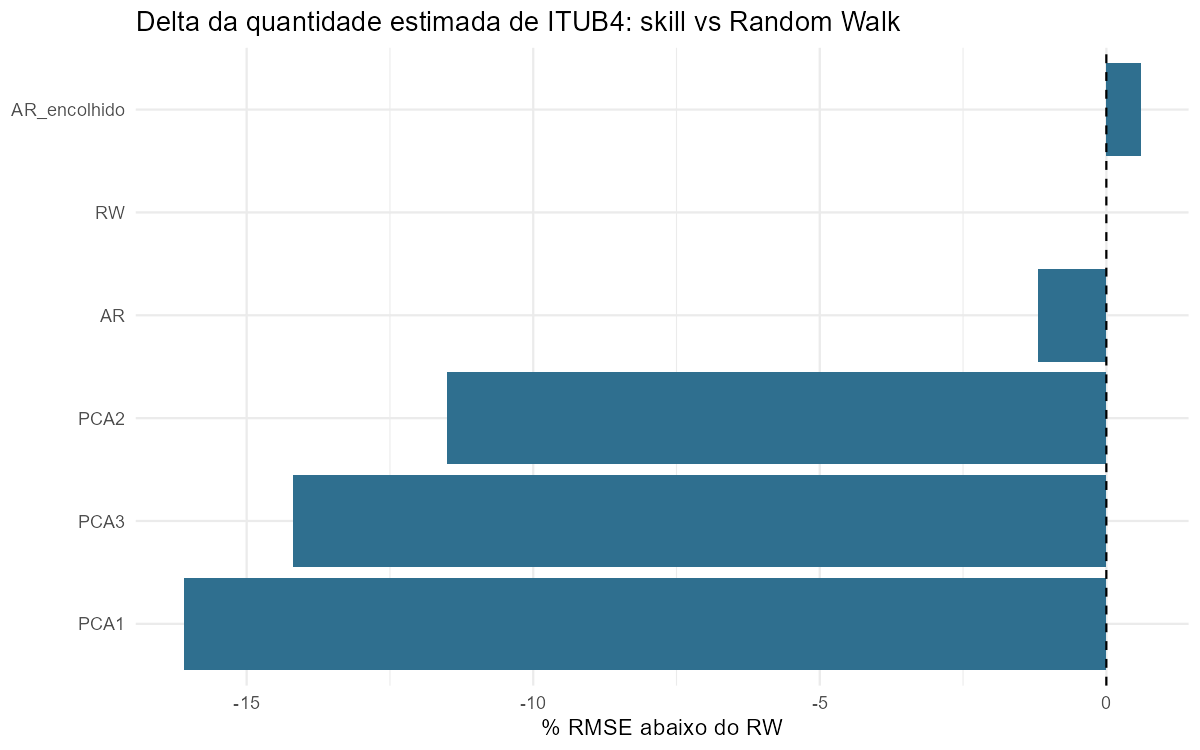
\includegraphics[width=0.76\textwidth]{forecast_quantity_delta_skill.png}
\caption{\emph{Skill} de RMSE para a variação mensal da quantidade estimada de ITUB4.}
\label{fig:qdelta}
\end{figure}

A leitura é que a variação mensal, tanto em valor quanto em quantidade aproximada, é difícil de prever com
modelos lineares simples. Esse resultado não encerra a pergunta; ele motiva olhar para o nível da exposição,
para janelas de previsão maiores e para informação adicional de mercado. O ponto estatístico, porém, é
claro: nos testes mensais de variação, nenhum modelo entrega melhora robusta sobre o \emph{random walk}.

\section{Previsão do nível e reversão à média}

Ao mudar o alvo para o nível da posição em valor, aparece previsibilidade. Para ITUB4, o AR individual reduz
o RMSE em cerca de 10\% contra o \emph{random walk} nos horizontes de 1 e 3 meses. O modelo de painel melhora
em horizontes mais longos, chegando a 9\% no horizonte de 6 meses. Esse resultado é relevante para risco
patrimonial, mas não deve ser interpretado automaticamente como previsibilidade de compras e vendas de
ações. A Tabela~\ref{tab:leveltests} torna a leitura mais precisa: em ITUB4, a magnitude da melhora em valor
é economicamente relevante, mas os testes pareados de perda não rejeitam igualdade contra o \emph{random
walk} nos níveis convencionais. Portanto, a conclusão correta não é ``o AR vence estatisticamente em
ITUB4'', e sim: ``ITUB4 sugere reversão à média em valor, que precisa ser checada em amostra mais ampla''.

\begin{table}[H]\centering
\caption{Nível de ITUB4: \emph{skill} de RMSE e teste de perda contra random walk.}
\label{tab:leveltests}
\scriptsize
\begin{tabular}{llrrrr}
\toprule
\textbf{Alvo} & \textbf{$h$} & \textbf{AR indiv.} & \textbf{$p$} &
\textbf{AR painel} & \textbf{$p$} \\
\midrule
Valor em US\$ & 1 & +10,0\% & 0,231 & +3,3\%  & 0,300 \\
Valor em US\$ & 3 & +10,2\% & 0,186 & +7,8\%  & 0,198 \\
Valor em US\$ & 6 & +7,1\%  & 0,461 & +9,0\%  & 0,298 \\
Quantidade    & 1 & +3,5\%  & 0,627 & -0,3\%  & 0,885 \\
Quantidade    & 3 & -2,6\%  & 0,642 & -1,6\%  & 0,690 \\
Quantidade    & 6 & -13,9\% & 0,067 & -11,1\% & 0,079 \\
\bottomrule
\end{tabular}
\begin{flushleft}
\scriptsize Nota: $h$ é o horizonte em meses. O $p$ testa a diferença de perda quadrática contra o
\emph{random walk}. Para quantidade, os horizontes de 3 e 6 meses pioram contra o benchmark.
\end{flushleft}
\end{table}

\begin{figure}[H]\centering
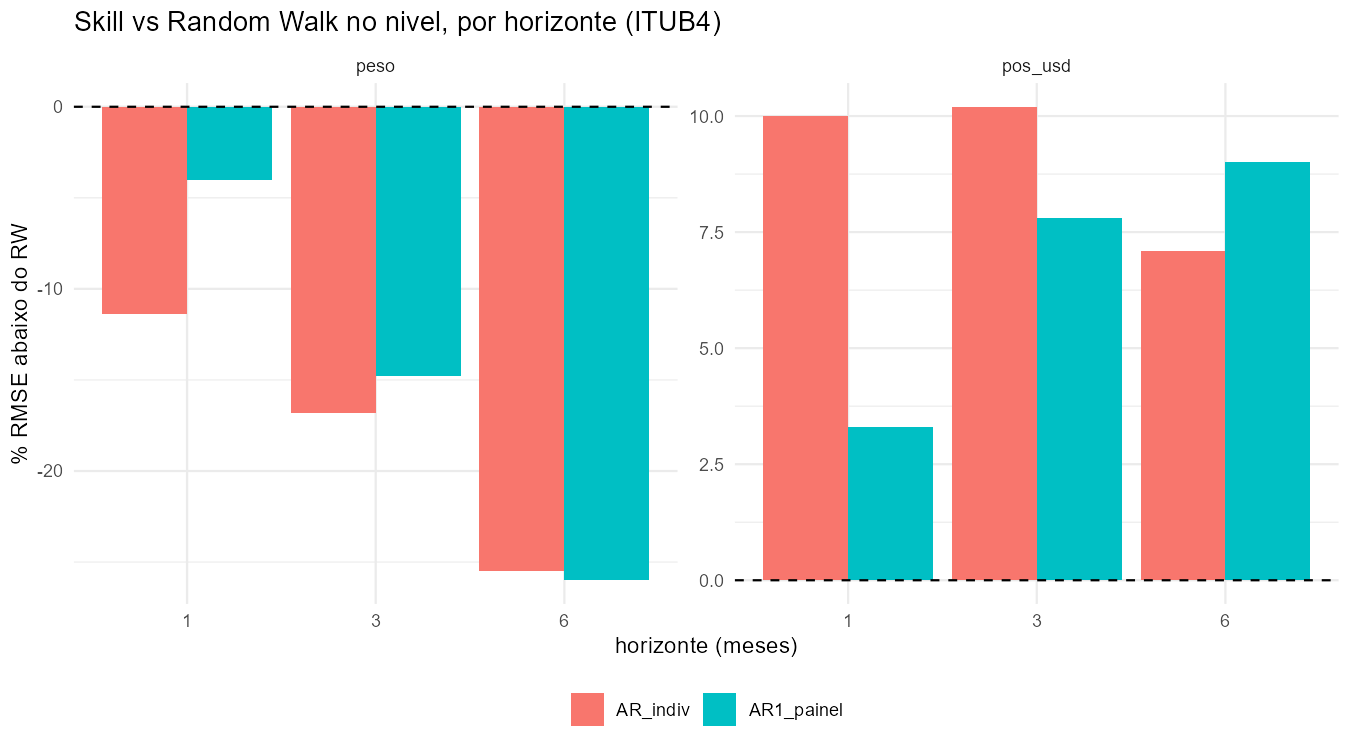
\includegraphics[width=0.88\textwidth]{forecast_round3_skill.png}
\caption{\emph{Skill} contra random walk no nível, por alvo e horizonte.}
\label{fig:r3}
\end{figure}

Como robustez, quando o alvo é o nível da quantidade estimada de ações, a evidência é mais fraca. O AR individual melhora o
RMSE em 3,5\% no horizonte de um mês, mas perde para o \emph{random walk} em três e seis meses. O modelo de
painel também não melhora a previsão. Portanto, a reversão em valor é mais forte do que a reversão em
quantidade.

\begin{figure}[H]\centering
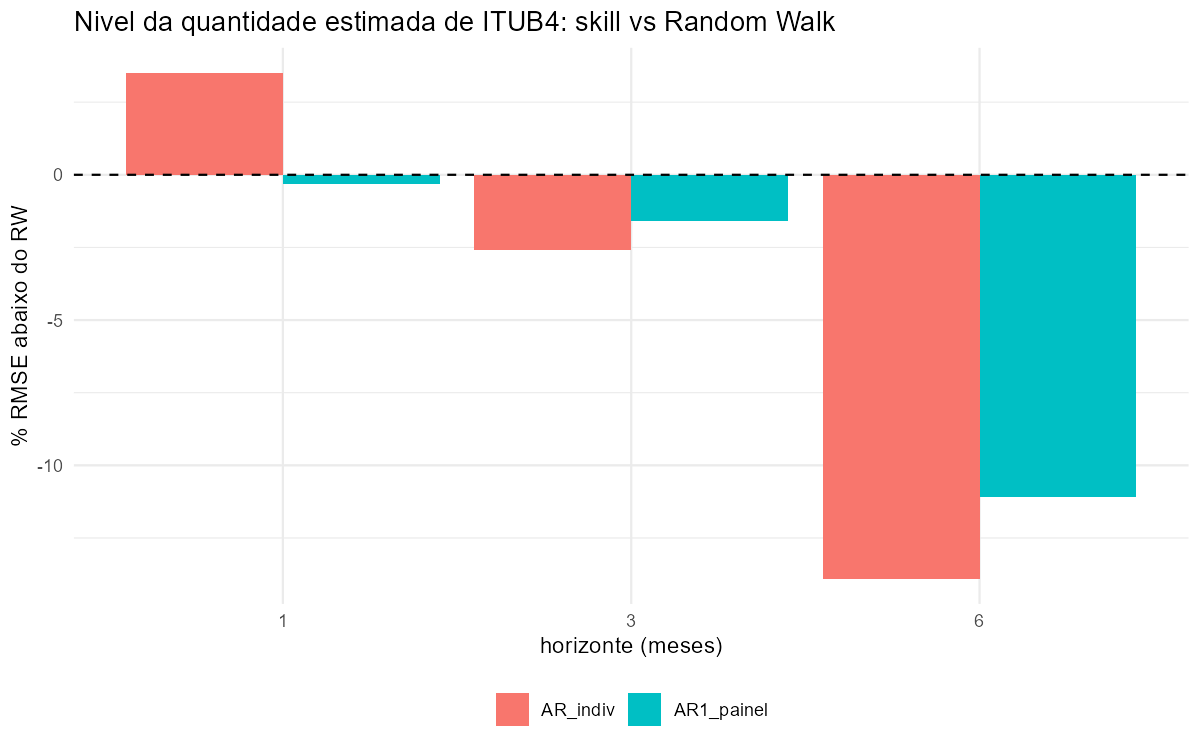
\includegraphics[width=0.76\textwidth]{forecast_quantity_level_skill.png}
\caption{\emph{Skill} contra random walk no nível da quantidade estimada de ITUB4.}
\label{fig:qlevel}
\end{figure}

O refinamento de meia-vida estima explicitamente a velocidade de retorno à alocação-alvo. Para a posição em
US\$ de ITUB4, 36 de 37 gestoras revertem à média; o coeficiente $\rho$ mediano é aproximadamente 0,77 e a
meia-vida mediana é 2,8 meses. Para a quantidade estimada, 33 de 37 gestoras revertem; o $\rho$ mediano sobe
para aproximadamente 0,83, a meia-vida mediana vai para 3,8 meses e a meia-vida de painel chega a 6,0 meses.
Isso sugere que a demanda em ações é mais persistente e menos previsível do que a exposição em valor.

\begin{table}[H]\centering
\caption{Meia-vida da reversão à alocação-alvo em ITUB4.}
\label{tab:halflife}
\scriptsize
\begin{tabular}{lrrrr}
\toprule
\textbf{Alvo} & \textbf{Revertem} & \textbf{$\rho$ med.} &
\textbf{MV med.} & \textbf{MV painel} \\
\midrule
Posição em US\$ & 36/37 & 0,77 & 2,8 meses & 2,6 meses \\
Quantidade estimada & 33/37 & 0,83 & 3,8 meses & 6,0 meses \\
\bottomrule
\end{tabular}
\end{table}

\begin{figure}[H]\centering
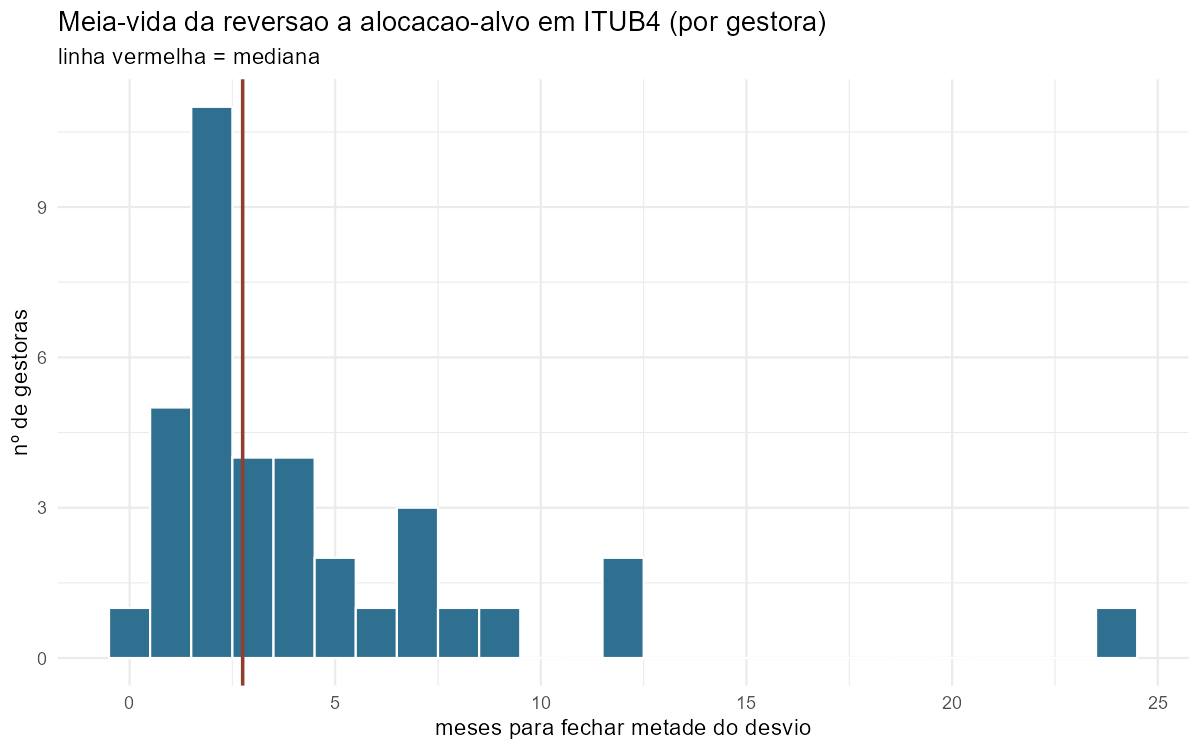
\includegraphics[width=0.76\textwidth]{half_life_hist.png}
\caption{Meia-vida da reversão à alocação-alvo em ITUB4.}
\label{fig:halflife}
\end{figure}

\begin{figure}[H]\centering
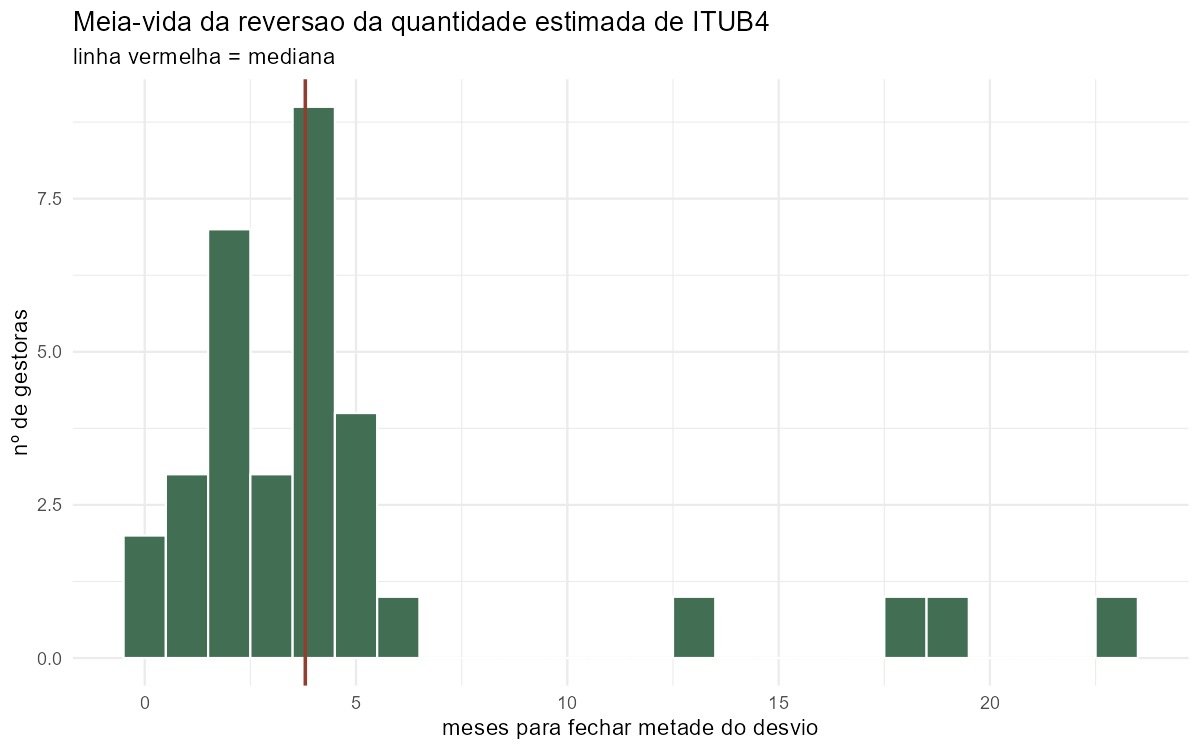
\includegraphics[width=0.76\textwidth]{half_life_quantity_hist.png}
\caption{Meia-vida da reversão da quantidade estimada de ITUB4.}
\label{fig:qhalflife}
\end{figure}

\section{Generalização do forecasting}

A rodada com todas as ações, ainda em valor, mostra que a previsibilidade do nível não é geral. O exercício
identifica 238 ações inicialmente avaliáveis; três são degeneradas para \emph{skill}, pois o \emph{random
walk} tem erro zero fora da amostra. A amostra válida, portanto, tem 235 ações. A mediana da \emph{skill} é
negativa e apenas 10,2\% das ações superam o \emph{random walk}. ITUB4 fica entre as melhores, com
\emph{skill} de 9,9\%, ao lado de PETR3 e ITSA4. Essa evidência deve ser lida como resultado de exposição
patrimonial; a generalização para quantidade exigiria baixar e validar preços mensais para todos os tickers.

\begin{table}[H]\centering
\caption{Generalização por ação: distribuição da skill do AR contra random walk.}
\label{tab:round5summary}
\small
\begin{tabular}{lr}
\toprule
\textbf{Métrica} & \textbf{Valor} \\
\midrule
Ações inicialmente avaliáveis & 238 \\
Tickers degenerados removidos & 3 \\
Ações válidas para skill & 235 \\
Skill mediana & -13,4\% \\
Ações com skill positiva & 10,2\% \\
Posição de ITUB4 no ranking & 3 de 235 \\
Skill de ITUB4 & +9,9\% \\
\bottomrule
\end{tabular}
\end{table}

\begin{table}[H]\centering
\caption{Ações com maior skill no forecast do nível em valor.}
\label{tab:round5top}
\small
\begin{tabular}{lrr}
\toprule
\textbf{Ticker} & \textbf{Gestoras} & \textbf{Skill RMSE} \\
\midrule
GOLL12 & 17 & +23,7\% \\
CGAS5  & 19 & +13,5\% \\
ITUB4  & 36 & +9,9\% \\
PETR3  & 35 & +9,7\% \\
ITSA4  & 34 & +9,6\% \\
\bottomrule
\end{tabular}
\end{table}

\begin{figure}[H]\centering
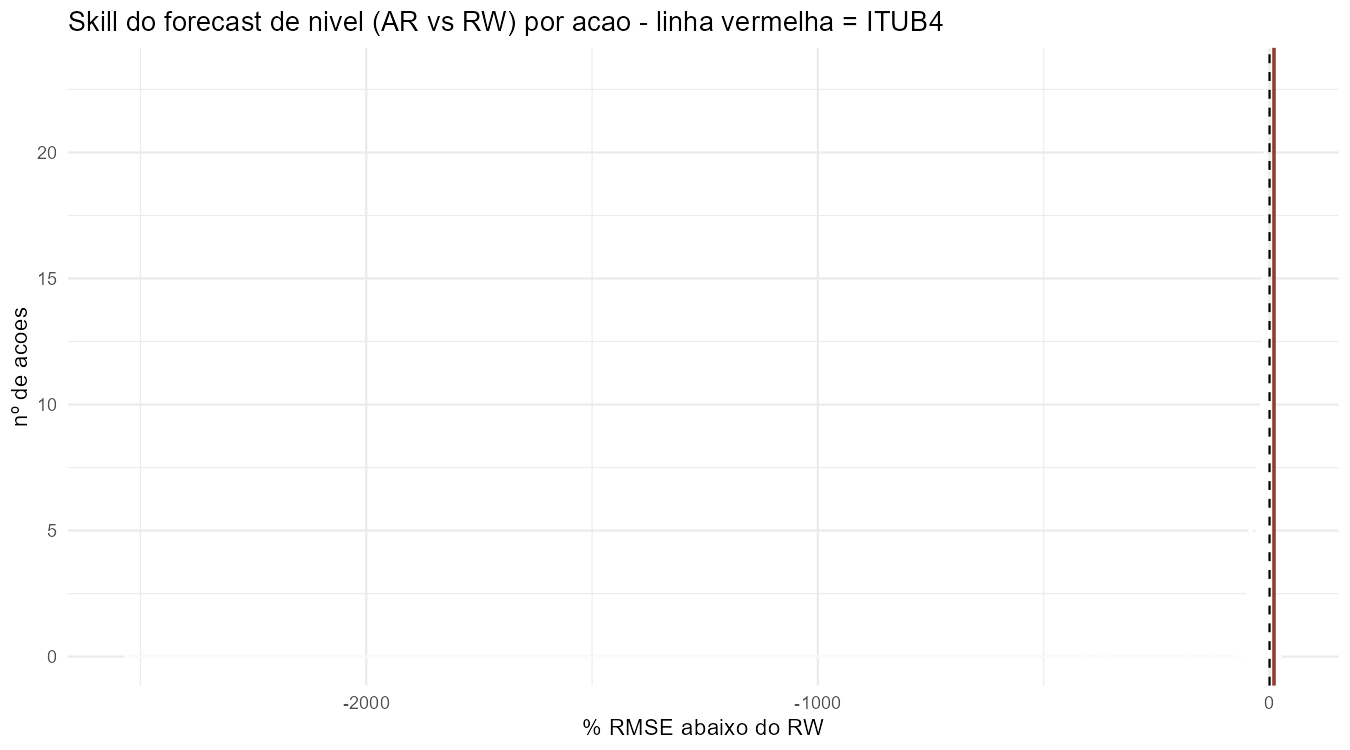
\includegraphics[width=0.82\textwidth]{forecast_round5_skill_hist.png}
\caption{Distribuição da \emph{skill} AR vs random walk por ação. Linha vermelha: ITUB4.}
\label{fig:r5}
\end{figure}

\section{Forecast consolidado com restante do mercado}

A especificação mais alinhada à pergunta final do TCC é o painel consolidado gestora $\times$ ação
$\times$ mês. Nessa versão, o alvo é $E_{g,i,t+1}$, o nível da exposição em US\$ da gestora $g$ na ação
$i$. O modelo usa não apenas o histórico da própria gestora, mas também o restante do mercado naquela ação:
a exposição média das demais gestoras, isto é, o componente $n-1$. Também é testado um fator comum de
exposição estimado por PCA apenas na janela de treino.

Após remover três tickers degenerados, em que o \emph{random walk} tem erro zero na amostra fora da amostra,
a avaliação contém 235 ações e 183.924 previsões por modelo. A Tabela~\ref{tab:consolforecast} mostra que o
\emph{random walk} continua sendo o benchmark mais difícil. AR individual, AR de painel, $n-1$ e fator comum
ficam levemente piores em RMSE e MAE. O coeficiente mediano do componente $n-1$ é 0,0054, praticamente zero,
e o coeficiente mediano do fator comum é 0,0009. O \emph{bootstrap} por mês não indica melhora
estatisticamente robusta de nenhum modelo contra o \emph{random walk}; em todos os casos, o intervalo de
\emph{bootstrap} da melhora média cruza zero.

\begin{table}[H]\centering
\caption{Forecast consolidado do nível da exposição em US\$ para todas as ações elegíveis.}
\label{tab:consolforecast}
\scriptsize
\begin{tabular}{lrrrrr}
\toprule
\textbf{Modelo} & \textbf{RMSE} & \textbf{MAE} & \textbf{Skill RMSE} &
\textbf{Direção} & \textbf{$p$ boot.} \\
\midrule
Random walk     & 10.752 & 2.638 & 0,00\%  & --     & -- \\
AR1 painel      & 10.855 & 2.786 & -0,96\% & 51,9\% & 0,777 \\
$n-1$ painel    & 10.869 & 2.869 & -1,09\% & 51,0\% & 0,814 \\
AR1 individual  & 10.870 & 2.821 & -1,10\% & 51,9\% & 0,778 \\
Fator comum     & 10.874 & 2.878 & -1,14\% & 51,0\% & 0,829 \\
\bottomrule
\end{tabular}
\begin{flushleft}
\scriptsize Nota: RMSE e MAE em US\$ milhões. $N=183.924$ previsões por modelo. O $p$ bootstrap testa
melhora sobre o \emph{random walk} reamostrando por data de origem; valores altos indicam ausência de
melhora robusta.
\end{flushleft}
\end{table}

\begin{figure}[H]\centering
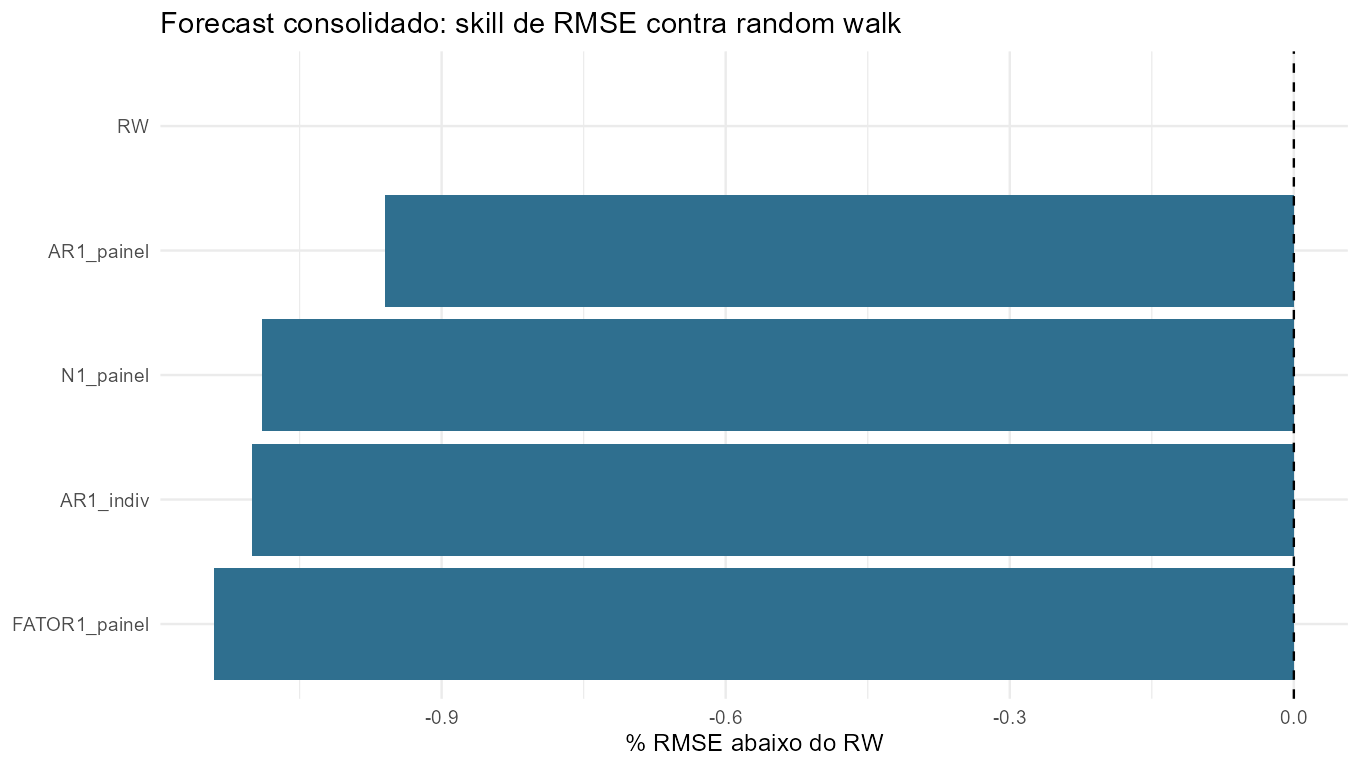
\includegraphics[width=0.78\textwidth]{forecast_consolidated_panel_skill.png}
\caption{\emph{Skill} de RMSE no forecast consolidado, contra o random walk.}
\label{fig:consolforecast}
\end{figure}

A conclusão é mais conservadora do que a evidência isolada de ITUB4. Em ITUB4, há reversão à média do nível
em valor. No painel amplo, porém, essa regularidade não se transforma em ganho agregado robusto. Isso é
coerente com a literatura de demanda: carteiras observadas revelam exposição e concentração institucional,
mas isso não implica que ajustes mensais agregados sejam facilmente previsíveis fora da amostra. Para o TCC,
esse resultado é importante porque evita uma narrativa excessivamente otimista. O projeto mede demanda
institucional com boa granularidade, mostra onde há concentração e testa previsibilidade com um benchmark
forte. A evidência final é que, no agregado, o \emph{random walk} permanece difícil de bater.

\section{Teste complementar com rede}

Uma especificação complementar adiciona a exposição dos vizinhos no grafo CDA como preditor do nível da
posição. O resultado não melhora o baseline de reversão à média: AR1 de painel tem \emph{skill} de 3,3\%,
enquanto o modelo com rede tem 3,1\%. Esse resultado deve ser lido com cautela. Ele não descarta o uso de
redes; mostra apenas que uma feature manual simples, baseada em média de vizinhos, não basta para superar o
AR de painel. Como a previsão principal é consolidada, esse teste é apresentado como extensão: o próximo
passo metodológico seria comparar uma versão com grafo, usando CDA e restante do mercado, contra os baselines
consolidados já estimados.

\chapter{Conclusão}

O projeto entrega cinco conclusões principais. Primeiro, é possível construir um painel mensal coerente de
exposição consolidada das gestoras a ações usando CONS e SH, com tratamento cuidadoso de formato numérico,
empréstimos de ações, grupos econômicos, R\$ e US\$. Segundo, a exposição institucional é concentrada em
\emph{blue chips}, o que conecta o exercício à literatura de demanda por ações e fragilidade por propriedade
comum. Terceiro, a variação mensal da exposição é difícil de prever com modelos lineares simples; o
\emph{random walk} é um benchmark forte. Quarto, o nível da exposição em valor apresenta reversão à média em
ITUB4 e em algumas ações muito líquidas, mas o forecast consolidado com todas as ações elegíveis, restante do
mercado e fator comum não supera o \emph{random walk}. Quinto, a quantidade estimada mostra que parte da
reversão patrimonial em valor não deve ser confundida com compra e venda previsível de ações.

A interpretação econômica é alinhada à literatura de demanda por ações. Carteiras observadas revelam demanda
institucional e permitem estudar quem aumenta ou reduz exposição em cada ação. Ao mesmo tempo, a estrutura de
fundos interconectados adiciona uma dimensão de risco, documentada no apêndice CDA: a exposição final pode
passar por estruturas FIC/master e por camadas de fundos sobre fundos. Portanto, o caminho natural do TCC é
um sistema de previsão consolidada de exposição por gestora e ação, usando histórico próprio e restante do
mercado como núcleo; a rede entra como extensão para enriquecer features e interpretar risco.

O resultado negativo da feature manual de rede não fecha a questão. Ele funciona como baseline: uma média de
vizinhos não acrescenta sinal suficiente, e a especificação consolidada com $n-1$ e fator comum também não
supera o \emph{random walk}. Um modelo de grafo mais flexível, como uma GNN temporal, ainda é
metodologicamente coerente como extensão, mas só seria defensável se mantivesse a mesma disciplina
fora-da-amostra: origem móvel, features estimadas apenas no treino, comparação contra \emph{random walk},
AR, painel, $n-1$ e fatores, e relatório explícito de quando o ganho não aparece.

\appendix
\chapter{Apêndice: CDA e Estruturas Fundo-Sobre-Fundo}\label{ap:cda}

\section{Por que a CDA aparece no projeto}

A CONS é consolidada: ela mostra os ativos finais da carteira, mas apaga relações entre fundos. Se um FIC
investe em um master que detém ações, a CONS mostra a exposição final em ações. Isso é ótimo para medir
exposição consolidada, que é o núcleo do TCC. Porém, isso é insuficiente para estudar a estrutura
fundo$\to$fundo. A CDA Bloco~2 entra somente para esse segundo objetivo: reconstruir a rede de cotas de
fundos, avaliar se há circularidade, medir profundidade de aninhamento e produzir uma base auditável para
extensões de graph learning.

Essa distinção é essencial. O TCC não depende da CDA para medir exposição em ITUB4, para construir o painel
gestora $\times$ ação $\times$ mês, nem para rodar os baselines principais de forecasting. O alvo principal
também não é prever a rede. O alvo é prever exposição consolidada. O grafo CDA é uma camada auxiliar para
entender a estrutura dos fundos e, no futuro, usar essa estrutura como informação adicional.

\section{O que é a CDA Bloco 2}

A CDA é a Composição e Diversificação das Aplicações dos fundos. O Bloco~2 registra cotas de fundos de
investimento. As colunas relevantes usadas no projeto são:
\begin{itemize}
\item \texttt{CNPJ\_FUNDO}: fundo que detém cotas;
\item \texttt{CNPJ\_FUNDO\_COTA}: fundo investido;
\item \texttt{DT\_COMPTC}: data de competência;
\item \texttt{VL\_MERC\_POS\_FINAL}: valor de mercado da posição;
\item \texttt{DT\_CONFID\_APLIC}: campo associado à confidencialidade de aplicação.
\end{itemize}

Nos arquivos históricos processados, \texttt{DT\_CONFID\_APLIC} aparece preenchido em 32,3\% das arestas,
mas \texttt{CNPJ\_FUNDO\_COTA} está disponível e destino vazio é zero. Portanto, o projeto não trata esse
campo como sinônimo de destino mascarado.

\section{Por que uma leitura simples da CDA fica ruim}

Uma tentativa como \texttt{read\_csv("C:/Users/joaoz/Downloads/CDA/cad\_fi.csv")} não reproduz o tratamento
usado aqui por três motivos.

Primeiro, o arquivo relevante para a rede não é um cadastro genérico de fundos, mas o arquivo histórico
anual do documento CDA, especificamente o arquivo do Bloco~2 dentro dos ZIPs anuais da CVM. Segundo, os
arquivos da CVM usam separador ponto-e-vírgula e encoding
\texttt{latin1}; por isso, uma leitura automática com vírgula pode quebrar colunas, acentos e tipos. Terceiro,
o arquivo bruto contém muito mais informação do que o necessário. O projeto seleciona apenas as colunas
necessárias para construir arestas fundo$\to$fundo e filtra a origem para fundos pertencentes ao universo
CONS+SH.

O tratamento usado no projeto está em \texttt{R/10\_build\_cda\_edges.R}. A sequência é:
\begin{enumerate}
\item baixar, quando necessário, os ZIPs anuais da CVM para 2016--2021;
\item abrir de dentro do ZIP o arquivo \texttt{cda\_fi\_BLC\_2\_AAAA.csv}, sem extrair todo o ZIP para disco;
\item ler o conteúdo com \texttt{sep=";"} e encoding \texttt{latin1};
\item selecionar as cinco colunas essenciais: fundo de origem, data, valor de mercado, fundo investido e
campo de confidencialidade;
\item normalizar CNPJs para 14 dígitos;
\item converter \texttt{DT\_COMPTC} para data e \texttt{VL\_MERC\_POS\_FINAL} para número;
\item manter apenas arestas cuja origem aparece no universo de fundos do projeto;
\item marcar se o destino também pertence ao universo CONS+SH.
\end{enumerate}

A saída processada é \texttt{data/processed/cda\_edges.csv}, com uma linha por posição fundo$\to$fundo
observada no Bloco~2. As colunas finais são:
\[
\{\texttt{ano},\texttt{data},\texttt{cnpj\_fundo},\texttt{cnpj\_cota},\texttt{valor\_brl},
\texttt{confidencial},\texttt{dentro\_universo}\}.
\]

\section{Construção da base processada}

O filtro de origem é deliberado. O objetivo não é reconstruir todo o sistema brasileiro de fundos, mas a
rede relevante para os fundos presentes no painel CONS+SH do TCC. Assim, \texttt{cnpj\_fundo} precisa estar
no universo do projeto. Já \texttt{cnpj\_cota} pode estar dentro ou fora desse universo. Quando o destino
está fora, a aresta ainda é economicamente informativa, mas não permite recuperar gestora, PL e exposição
final no mesmo painel.

A Tabela~\ref{tab:cdaresumo} resume a massa de dados por ano. O crescimento do número de arestas é
compatível com a expansão do universo observado e com maior densidade de estruturas fundo-sobre-fundo.

\begin{table}[H]\centering
\caption{Resumo da CDA processada.}
\label{tab:cdaresumo}
\small
\begin{tabular}{rrrrr}
\toprule
\textbf{Ano} & \textbf{Arestas} & \textbf{DT\_CONFID} & \textbf{Destino no universo} & \textbf{Destino externo} \\
\midrule
2016 & 100.824 & 22.079 & 34.212 & 66.612 \\
2017 & 105.717 & 31.805 & 35.024 & 70.693 \\
2018 & 115.763 & 38.549 & 38.215 & 77.548 \\
2019 & 133.670 & 50.980 & 44.651 & 89.019 \\
2020 & 166.317 & 59.650 & 55.406 & 110.911 \\
2021 & 213.403 & 67.105 & 67.389 & 146.014 \\
\bottomrule
\end{tabular}
\end{table}

\section{Validação da CDA}

As principais checagens foram feitas antes de usar a CDA para qualquer interpretação econômica:
\begin{itemize}
\item \textbf{identidade das arestas}: a aresta é sempre lida como fundo de origem detendo cotas do fundo de
destino;
\item \textbf{CNPJ}: origem e destino são normalizados com a mesma função usada no restante do projeto;
\item \textbf{datas}: a competência é mensal e compatível com os painéis CONS+SH;
\item \textbf{valores}: \texttt{valor\_brl} está em reais, não em mil reais;
\item \textbf{self-loops}: não há fundo investindo diretamente nele mesmo;
\item \textbf{duplicatas}: não há duplicatas exatas de arestas no arquivo processado;
\item \textbf{valores inválidos}: os valores de mercado não têm NAs nem valores negativos;
\item \textbf{confidencialidade}: \texttt{DT\_CONFID\_APLIC} preenchido não é tratado automaticamente como
destino mascarado, porque \texttt{CNPJ\_FUNDO\_COTA} permanece preenchido;
\item \textbf{fração de propriedade}: quando há PL do destino, calcula-se
$\phi=\text{valor}/PL_{\text{destino}}$ para avaliar plausibilidade.
\end{itemize}

A fração $\phi$ tem mediana próxima de 0,007 e a grande maioria das observações com PL válido fica em
$(0,1]$. Casos com $\phi>1$ são raros e foram capados em 1 no cálculo de de-duplicação. Isso é conservador:
impede que erro de unidade, defasagem de PL ou diferença de cobertura gere propriedade acima de 100\%.

\section{Visualização dos grafos}

As figuras de rede são geradas por \texttt{R/21\_cda\_graph\_figures.R}. Elas não são desenhos manuais:
partem de \texttt{data/processed/cda\_edges.csv}. A Figura~\ref{fig:cdafundgraph} mostra o subgrafo
fundo$\to$fundo mais conectado em dezembro de 2021, filtrado para os 120 nós de maior grau e removendo
isolados. Nós azuis são fundos no universo CONS+SH; nós cinza são origens ou destinos fora do universo
principal, mas observados na CDA.

\begin{figure}[H]\centering
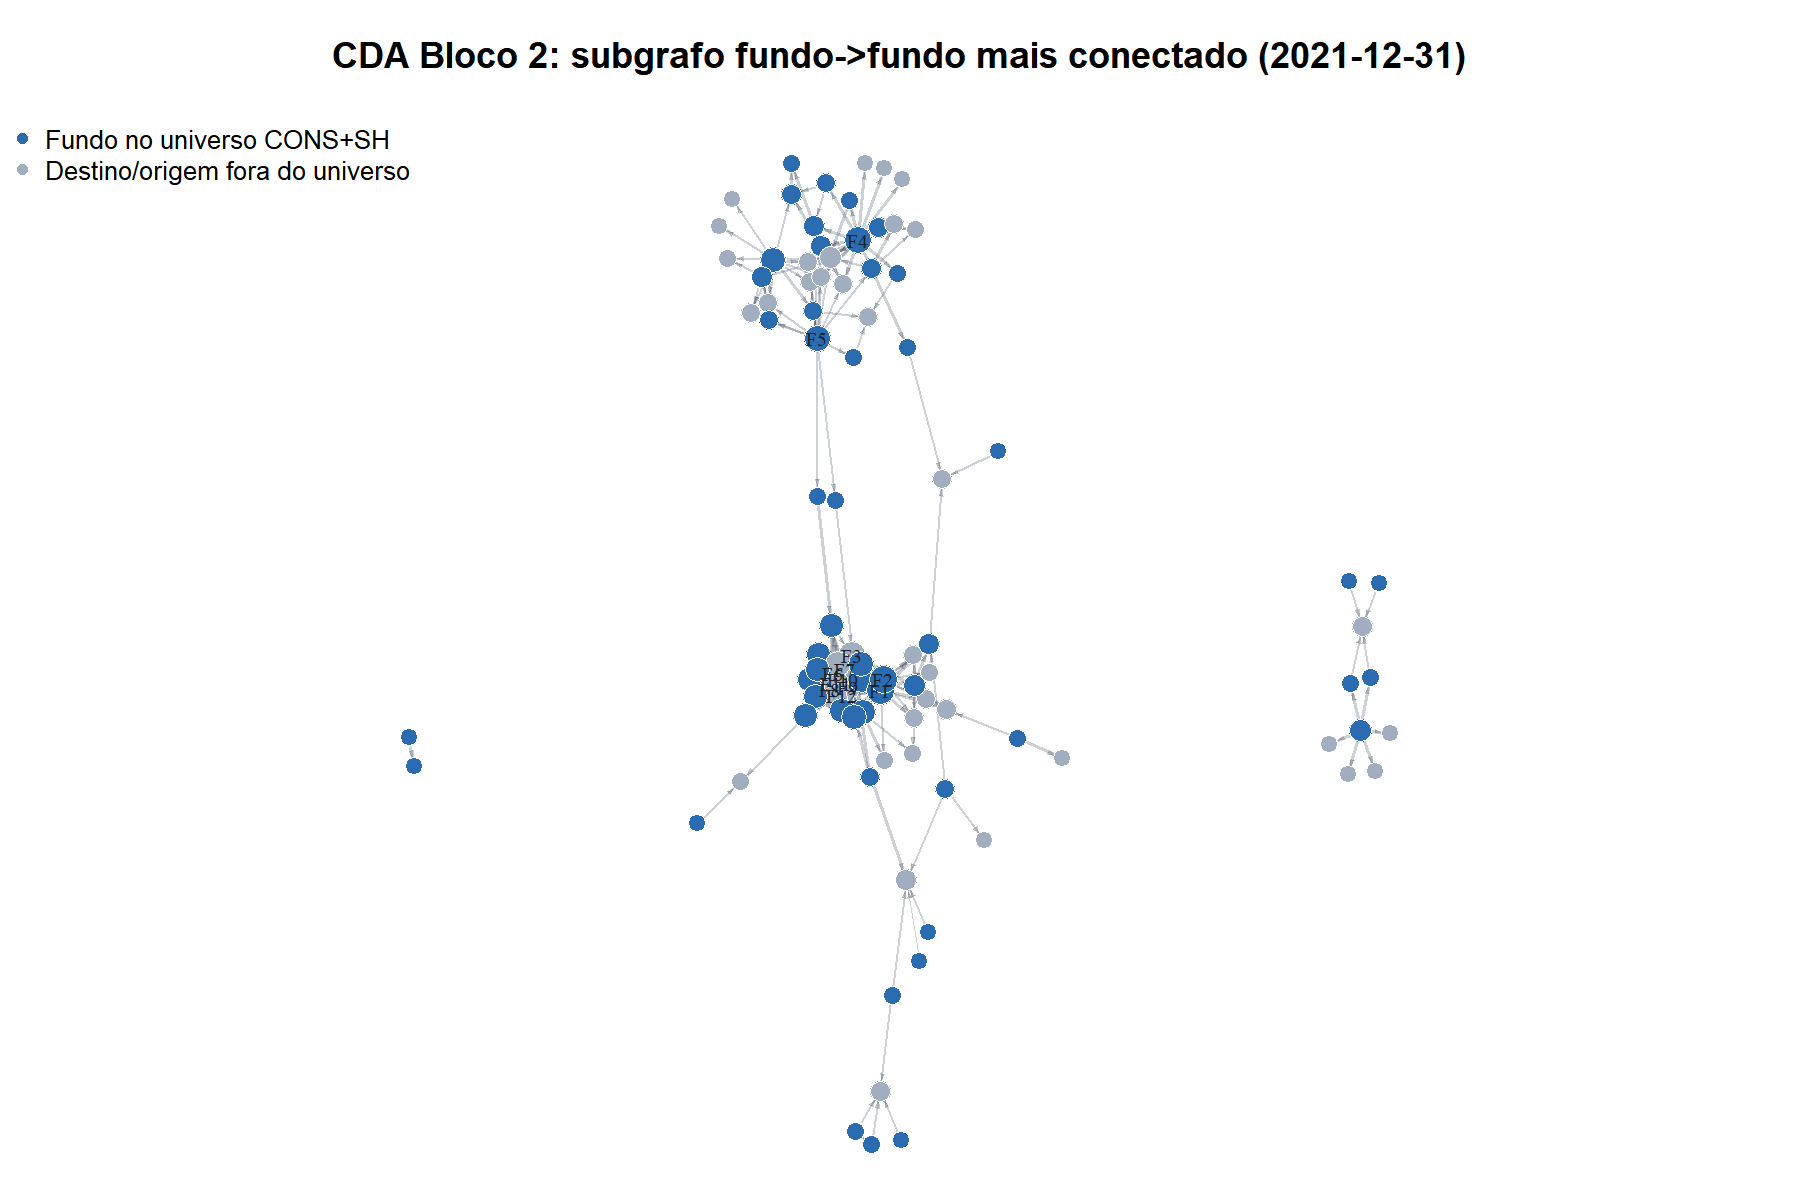
\includegraphics[width=0.92\textwidth]{cda_graph_fund_core.png}
\caption{CDA Bloco 2: subgrafo fundo$\to$fundo mais conectado em dezembro de 2021.}
\label{fig:cdafundgraph}
\end{figure}

A Figura~\ref{fig:cdamgrgraph} projeta as arestas para o nível de gestoras: uma aresta gestora A
$\to$ gestora B aparece quando fundos da gestora A detêm cotas de fundos da gestora B. Essa figura usa
apenas arestas entre casas diferentes, para evitar que auto-laços dominem visualmente a rede. Ela não é a
base do forecasting principal; serve para mostrar que há interconexões observáveis entre estruturas de
fundos.

\begin{figure}[H]\centering
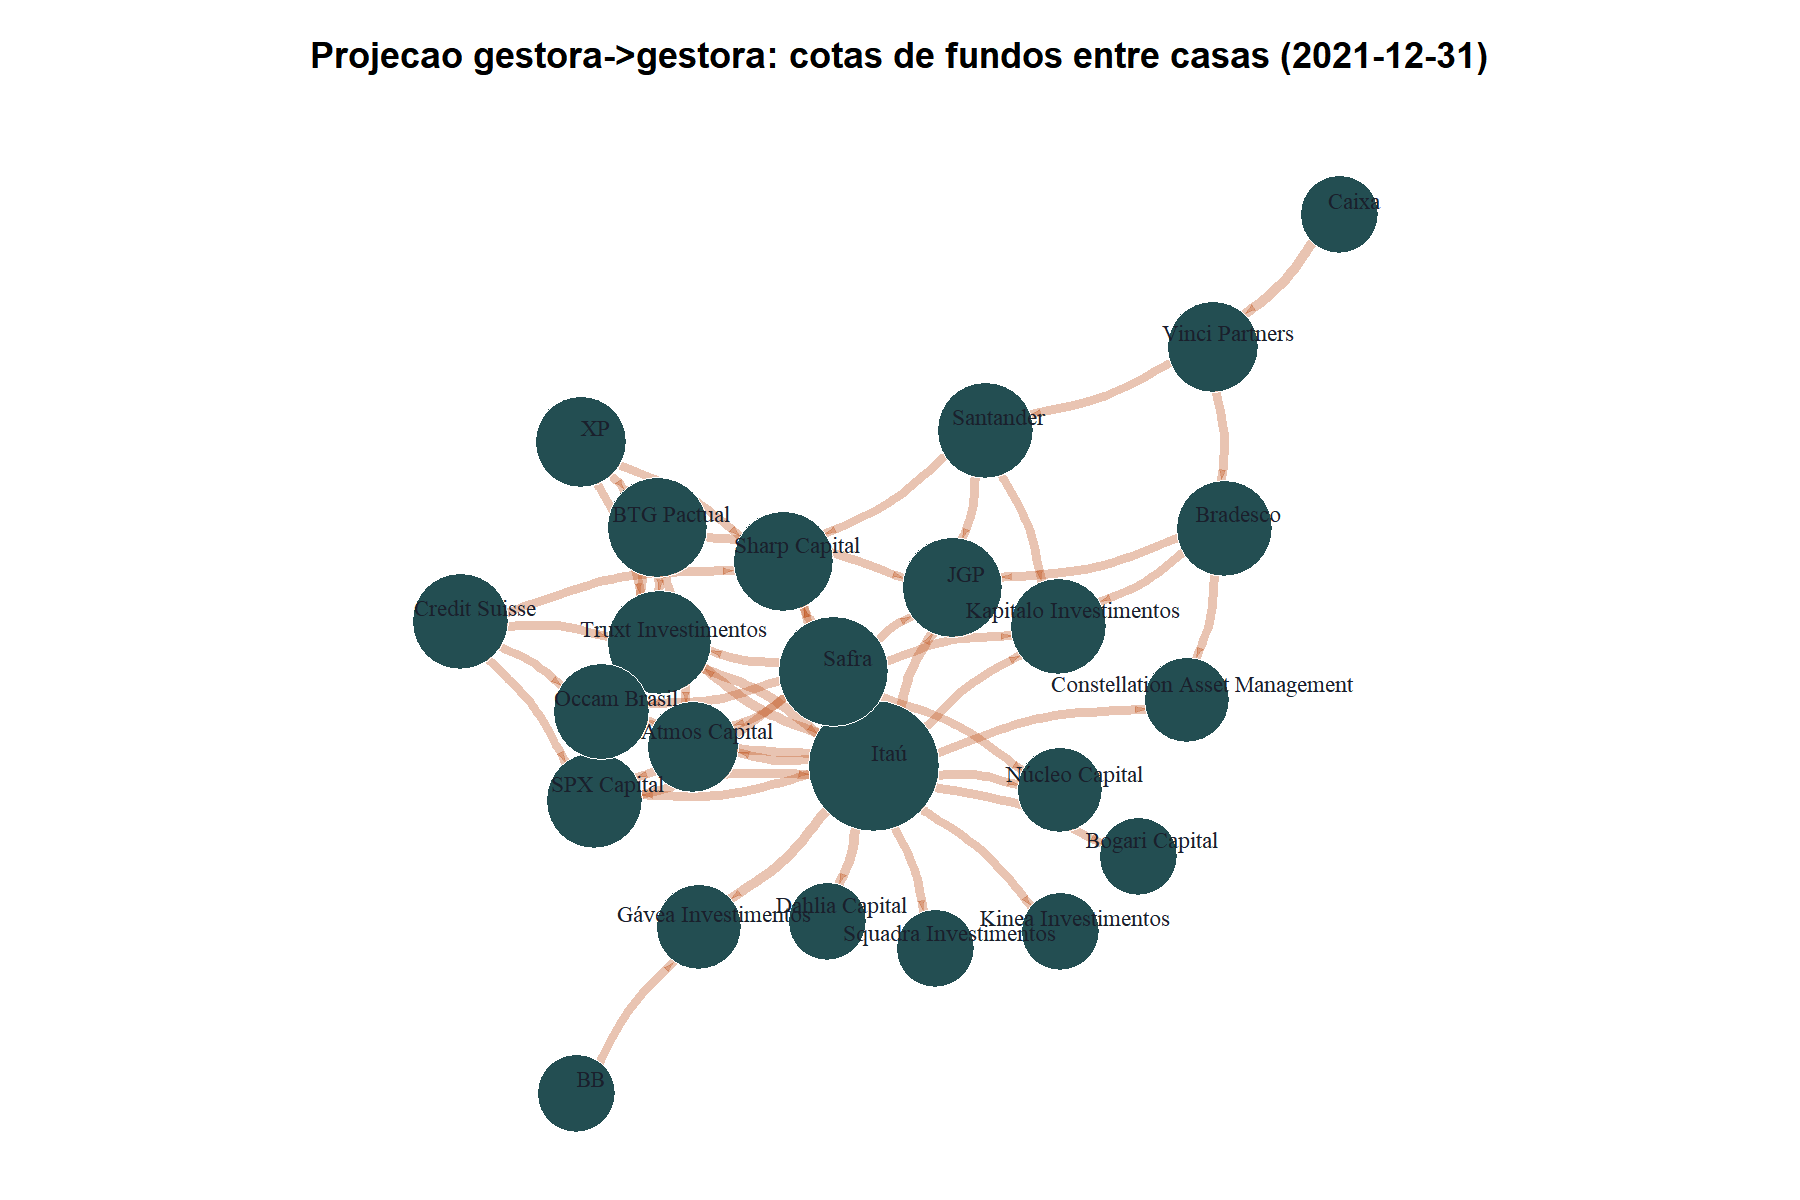
\includegraphics[width=0.92\textwidth]{cda_graph_manager_projection.png}
\caption{Projeção gestora$\to$gestora das cotas de fundos entre casas em dezembro de 2021.}
\label{fig:cdamgrgraph}
\end{figure}

No mês de referência usado nas figuras, a CDA processada contém 5.045 nós e 19.191 arestas antes do filtro
visual. O subgrafo visualizado tem 96 nós e 258 arestas. A projeção por gestora mostra 45 arestas
intergestoras entre 38 grupos, após selecionar as maiores relações por valor.

\section{Ciclos e profundidade}

Uma preocupação natural em estruturas FIC/master é a existência de circularidade: fundo A investe em B, B em
C e C volta a A. Essa situação dificultaria a interpretação de exposição look-through. Para testar isso, o
projeto constrói, mês a mês, o subgrafo de arestas em que origem e destino estão no universo CONS+SH e usa
\texttt{igraph::is\_dag}. O resultado é: todos os 72 meses são DAGs. Portanto, não encontramos ciclos
diretos no subgrafo observado.

Ausência de ciclos não significa ausência de complexidade. O mesmo módulo mede a maior cadeia direcionada em
cada mês. A profundidade máxima tem mediana 7 e máximo 9 níveis. Isso indica estruturas de aninhamento
relevantes: a exposição final pode passar por várias camadas de fundos antes de chegar ao ativo consolidado.

\begin{table}[H]\centering
\caption{Estrutura da rede CDA no universo observado.}
\small
\begin{tabular}{lr}
\toprule
\textbf{Métrica} & \textbf{Valor} \\
\midrule
Arestas CDA processadas & 835.694 \\
Meses analisados & 72 \\
Meses com ciclos & 0 \\
Profundidade máxima mediana & 7 \\
Profundidade máxima observada & 9 \\
Nós no último mês, subgrafo intra-amostra & 2.565 \\
Arestas no último mês, subgrafo intra-amostra & 5.968 \\
\bottomrule
\end{tabular}
\end{table}

\section{De-duplicação intra-gestora}

Se o fundo A de uma gestora investe no fundo B da mesma gestora, e B tem exposição $L_B$ a uma ação, parte
de $L_B$ pode aparecer duas vezes quando somamos fundos da gestora. A fração de B detida por A é:
\[
\phi_{A\to B} = \frac{v_{A\to B}}{PL_B}.
\]
Assim, a exposição de-duplicada por gestora é:
\[
\text{dedup}_g = \sum_{i\in g} L_i -
\sum_{A\to B \in g} \phi_{A\to B}L_B.
\]

Para ITUB4, a duplicação intra-gestora estimada é 37,6\%. Se também forem consideradas arestas entre
gestoras no universo observado, a duplicação rastreável aumenta em cerca de 5,3 pontos percentuais, chegando
a 43,0\%. Portanto, o número de 37,6\% deve sempre ser lido como duplicação \emph{intra-gestora}, não como
duplicação total do sistema.

\begin{figure}[H]\centering
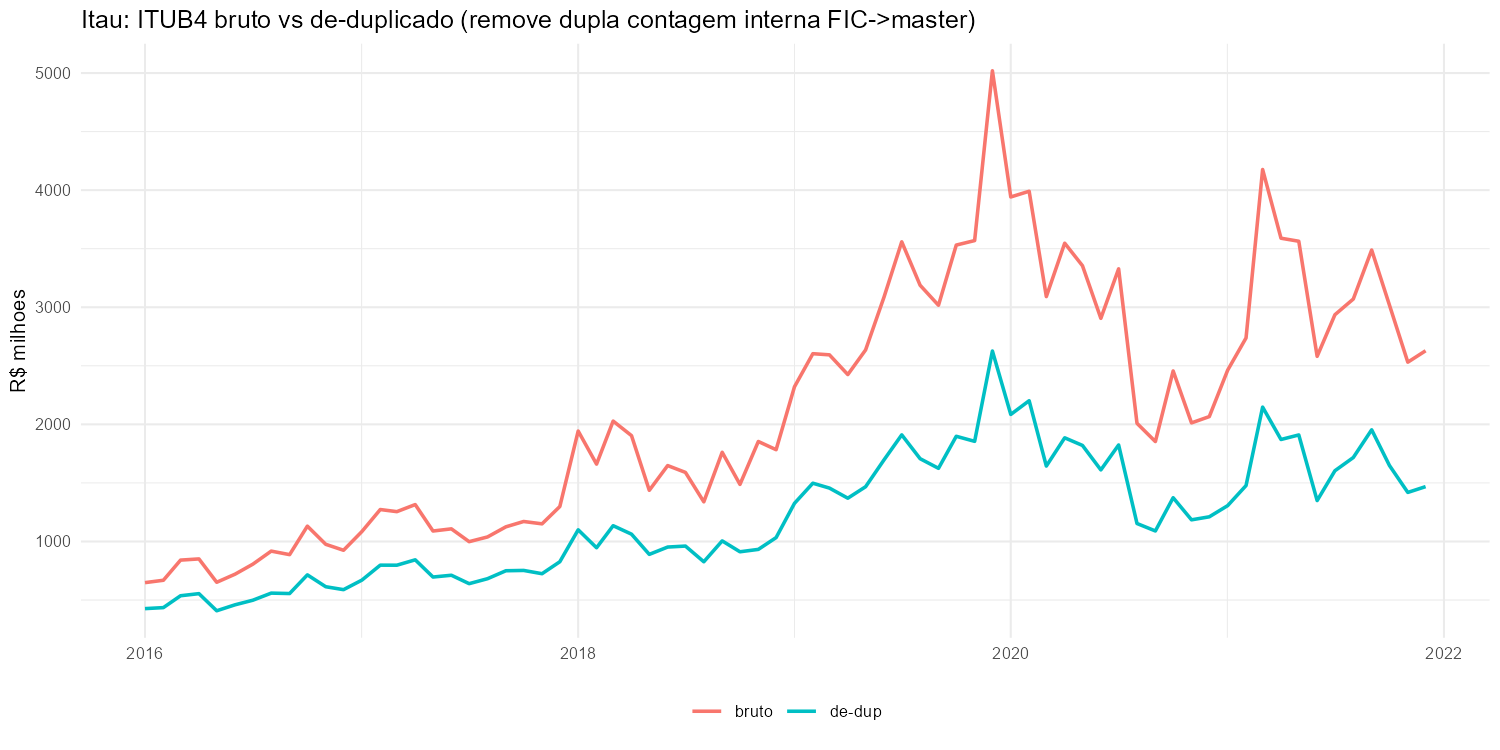
\includegraphics[width=0.84\textwidth]{itub4_dedup_itau.png}
\caption{Itaú: exposição bruta e de-duplicada em ITUB4.}
\label{fig:dedup}
\end{figure}

\section{Como a CDA se conecta a modelos de grafo}

É tentador dizer que o projeto ``prevê grafos'', mas essa não é a formulação correta no estágio atual. O que
o projeto prevê é exposição consolidada:
\[
\widehat{E}_{g,i,t+h}.
\]
O grafo entra como informação auxiliar. Em uma extensão, poderíamos escrever:
\[
\widehat{E}_{g,i,t+h}
= f(E_{g,i,\leq t}, E_{-g,i,\leq t}, G_t),
\]
em que $G_t$ é o grafo observado de fundos ou gestoras no mês $t$. Uma GNN usaria a matriz de adjacência
derivada da CDA e atributos dos nós, como exposição atual, variação passada, PL, centralidade, grau e
vizinhança. O alvo continuaria sendo exposição futura, não a aresta futura.

O teste já feito com feature manual de rede é uma versão fraca dessa ideia: usa a exposição dos vizinhos no
grafo como preditor adicional. O resultado não superou o AR de painel. Isso não prova que todo modelo de
grafo falhará; apenas mostra que uma média simples de vizinhos não captura sinal incremental suficiente. Para
ser defensável, qualquer GNN futura deve ser comparada contra \emph{random walk}, AR, painel e fatores,
sempre com origem móvel e sem vazamento.

\section{Limitações da CDA}

A CDA tem três limitações principais:
\begin{enumerate}
\item ela mede relações de cotas de fundos, não exposição final em ações; por isso deve ser usada junto com a
CONS, não em substituição a ela;
\item muitos destinos estão fora do universo CONS+SH usado no painel principal, o que limita a cobertura de
rede observável;
\item a interpretação de \texttt{DT\_CONFID\_APLIC} exige cautela e não deve ser descrita como destino
mascarado quando o CNPJ do destino está preenchido.
\end{enumerate}

Assim, a CDA deve ser tratada como apêndice técnico robusto: útil, auditado e visualmente informativo, mas
separado do núcleo consolidado. A conclusão principal do TCC não depende dela. A contribuição da CDA é
mostrar a estrutura de fundos sobre fundos que a CONS apaga, quantificar risco de aninhamento e deixar pronta
uma trilha metodológica para modelos de grafo.

\bibliographystyle{plainnat}
\bibliography{refs}
\end{document}
